\documentclass[11pt,a4paper]{article}
\usepackage{iftex}
\ifXeTeX
  \usepackage{xeCJK}
  \setCJKmainfont{FandolSong-Regular}
\else
  \usepackage{CJKutf8}
\fi

\usepackage[margin=1in]{geometry}
\usepackage{microtype}
\usepackage{graphicx}
\graphicspath{{figures/}}
\usepackage{booktabs}
\usepackage{array}
\usepackage{tabularx}
\usepackage{amsmath}
\usepackage{amssymb}
\usepackage[numbers]{natbib}
\usepackage{hyperref}
\hypersetup{colorlinks=true,linkcolor=blue,citecolor=blue,urlcolor=blue}
\newcommand{\sys}{LMPool}
\newcolumntype{L}[1]{>{\raggedright\arraybackslash}p{#1}}
\newcolumntype{Y}{>{\raggedright\arraybackslash}X}
\setlength{\emergencystretch}{3em}
\sloppy

\title{LMPool：面向多 GPU LLM 服务的局部性路由与 NVLink KV Cache 传输}
\author{Jialiang Li\\香港科技大学}
\date{}

\begin{document}
\ifXeTeX\else\begin{CJK*}{UTF8}{gbsn}\fi
\maketitle

\begin{abstract}
前缀缓存可以避免重复的 prefill 计算，但数据并行 LLM 副本的 KV cache 相互独立，
可复用状态可能位于并非当前选定 worker 的 GPU 上；而严格将请求路由到前缀 owner
又可能使该 GPU 过载。本文提出 \sys{}，一个 LLM serving 系统：它以 KV-aware
routing 解决 cache locality，以直接 NVLink transfer 在 KV 放置不再匹配需求时提供
cache fluidity。路由器在连续已就绪前缀复用、排队成本和容量成本之间进行权衡；pair-
和 payload-aware 成本模型仅在预测可节省的 prefill 时间足以覆盖 transfer 成本时，才
准许 copy 或 move 操作；版本化事务协议确保未完成的副本不会参与路由决策。在六张
RTX 3090 GPU 上，针对 Qwen3-0.6B 和 Qwen3-1.7B，5 倍共享前缀长度的 routing 相比
round-robin data parallelism，分别将吞吐提升 11.8\% 和 21.3\%，将平均 TTFT 降低
18.6\% 和 25.2\%，并将未缓存 prefill token 数降低 59.9\% 和 61.0\%。对所有 layer
的打包 K/V microbenchmark 验证了按 GPU pair 区分的 1--64-block transfer profile。
端到端实验验证了 background placement 以及 0.6B 中 move-style source release 的实现，
同时表明一次已完成的 transfer 本身并不必然带来更低的 E2E latency 或更高的 throughput。
源代码位于 \url{https://github.com/0x0addc001/LMPool}。
\end{abstract}

\section{引言}

PagedAttention~\citep{vLLM} 和 RadixAttention~\citep{SGLang} 使单个推理引擎中的
前缀复用成为现实。然而，多 GPU 部署通常在每张 GPU 上运行一个数据并行模型副本和
一个 cache allocator。物理 KV block 仍局部于各自副本，而请求则经由集群级入口到达。
这种分离产生了放置问题：输入 prompt 可能匹配已驻留在某张 GPU 上的前缀，但传统
round-robin dispatcher 可能将请求分配到另一张 GPU，选中的副本因而需要重新计算并
保存同一前缀。

全局 cache policy 有两种相反的失败方式。将每个匹配请求都路由到 prefix owner 会把
热点前缀的请求集中到一个副本，使其他副本利用不足并降低整体 batching efficiency。
不加区分地重新分发 KV block 则会产生通信、同步和内存干扰成本，即使本地重新计算更
便宜也是如此。因此，有效的策略必须让 request router 与 KV-cache placement mechanism
共享对 locality、load、capacity 和 topology 的一致视图。

\sys{} 遵循两条原则。Routing principle 解决 cache locality：当减少的 prefill work
大于额外的排队和容量压力时，请求应在已经保存相关 KV prefix 的 GPU 上执行；有效的
routing 也会减少后续数据移动。Transfer principle 解决 cache fluidity：当 KV placement
不再匹配请求负载时，直接 NVLink transfer 可将有用 block 移到可复用它的副本。Transfer
不解决任意 request skew；它解决 KV 放置不均和跨实例复用，否则这些情形只能依赖数据
移动或重新计算。

因此，系统在能够保持 locality 时优先 routing，只有数据移动既必要又有利时才使用最快
的受支持直接 transfer path。\sys{} 将多 GPU HBM 视为逻辑协调的 pool，而不是物理共享
内存。每个 worker 保留对本地 allocation 与 KV tensor 的所有权；control plane 只协调
metadata、reservation、routing decision 和 transfer transaction，不访问物理 KV 数据。

本文实现了 locality- 和 load-aware router，以及 cost-gated KV-transfer path。入口处的
router 在所有 healthy replica 中匹配连续完整 prefix block，并权衡节省的 prefill work
与 queueing、decode、capacity 和 reclamation cost。Transfer path 仅限直接 NVLink pair，
批量处理完整 block chain，支持 copy 与 move，并在显式 transaction 中使用 generation
check 和 rollback。实验通过三类受控 workload 区分稳定的 routing 收益、已验证的 transfer
机制，以及 transfer 无法摊销其成本的情况。

\section{背景与动机}

\subsection{Paged KV Caching}

自回归 decoding 会在每个 layer 为每个已处理 token 保存 key 和 value vector。
PagedAttention 将这些状态划分为固定大小的物理 block，并将每个 sequence 的逻辑 block
映射到物理 block~\citep{vLLM}。Prefix caching 对完整逻辑 block 做 hash，使具有相同
hash chain 的两个请求可以引用同一 ready physical block。Block-based allocation 减少
fragmentation，hash-based sharing 避免重复 prefill，但复用仍局限于拥有该物理 block 的
cache allocator。对被拆分为完整 block $b_0,\ldots,b_k$ 的 prompt，\sys{} 计算 chained hash：
\begin{equation}
  h_i = \mathrm{xxhash64}(h_{i-1} \parallel b_i),
\end{equation}
其中 $h_{-1}$ 为空。部分 tail block 不能全局复用。有效匹配必须从 $h_0$ 开始且保持连续；
孤立的后续 hash 不足以构成匹配，因为其 attention dependency 不存在。

\subsection{观察一：复用是放置属性}

只有请求在保存匹配 KV state 的 GPU 上执行，或者 transfer 该 state 比重新计算更便宜时，
prefix-cache hit 才有价值。Round-robin 下的独立副本可能保留许多本地 cache entry，却在
请求准入时无法使用它们。相反，global router 可在不增加物理 cache capacity 的情况下提升
request-level 与 token-level reuse。因此，应先考虑 routing，再考虑数据移动。

\subsection{观察二：局部性与负载均衡竞争}

长共享前缀往往对应大量请求。将每个匹配请求都送到第一个 owner 会将 locality 转化为
load hotspot。仅看 aggregate hit rate 无法暴露此问题，因此评估还必须包括每个 rank 的
request 数、token 数、prefill/decode time、GPU utilization 和 memory utilization。Routing
decision 需考虑剩余 prefill work、queued token、active decode work、free block 和
reclamation pressure；目标不是最大化 hit rate，而是最小化 expected completion cost。

\subsection{观察三：Transfer 必须覆盖其成本}

在评估节点上，直接 NVLink 比 host-mediated storage path 更快，但每次 transfer 都会
reserve destination block、同步两个 worker、消耗 link 与 memory bandwidth，并更新 control
metadata。短生命周期或冷 KV state 应重新计算或 evict，而非 transfer。当完整热点 chain
可能被复用、session 移到另一副本，或保留可复用状态能缓解实际 local block shortage 时，
transfer 才有吸引力。这一观察促成了 transfer batching、基于实测 bandwidth 的 cost
estimation，以及 foreground 与 background transfer 的独立 admission policy。

\subsection{范围}

\sys{} 面向同一模型在一台多 GPU 节点上的副本，直接 NVLink pair 可被显式配置或自动
发现。由于 ingress request 尚未分配给 worker，ingress routing 可选择任意 healthy replica。
Worker-originated rerouting 与所有 KV-transfer plan 则仅限当前 GPU 及其已配置 direct NVLink
partner；不相关的 PCIe 或 NUMA peer 不作为 transfer path。系统补充而非替代 RDMA-based
和 storage-tier system；cross-node RDMA、CPU/SSD tier、heterogeneous model 与透明 remote
memory addressing 不在当前范围内。

\section{系统设计}

\begin{figure*}[t]
  \centering
  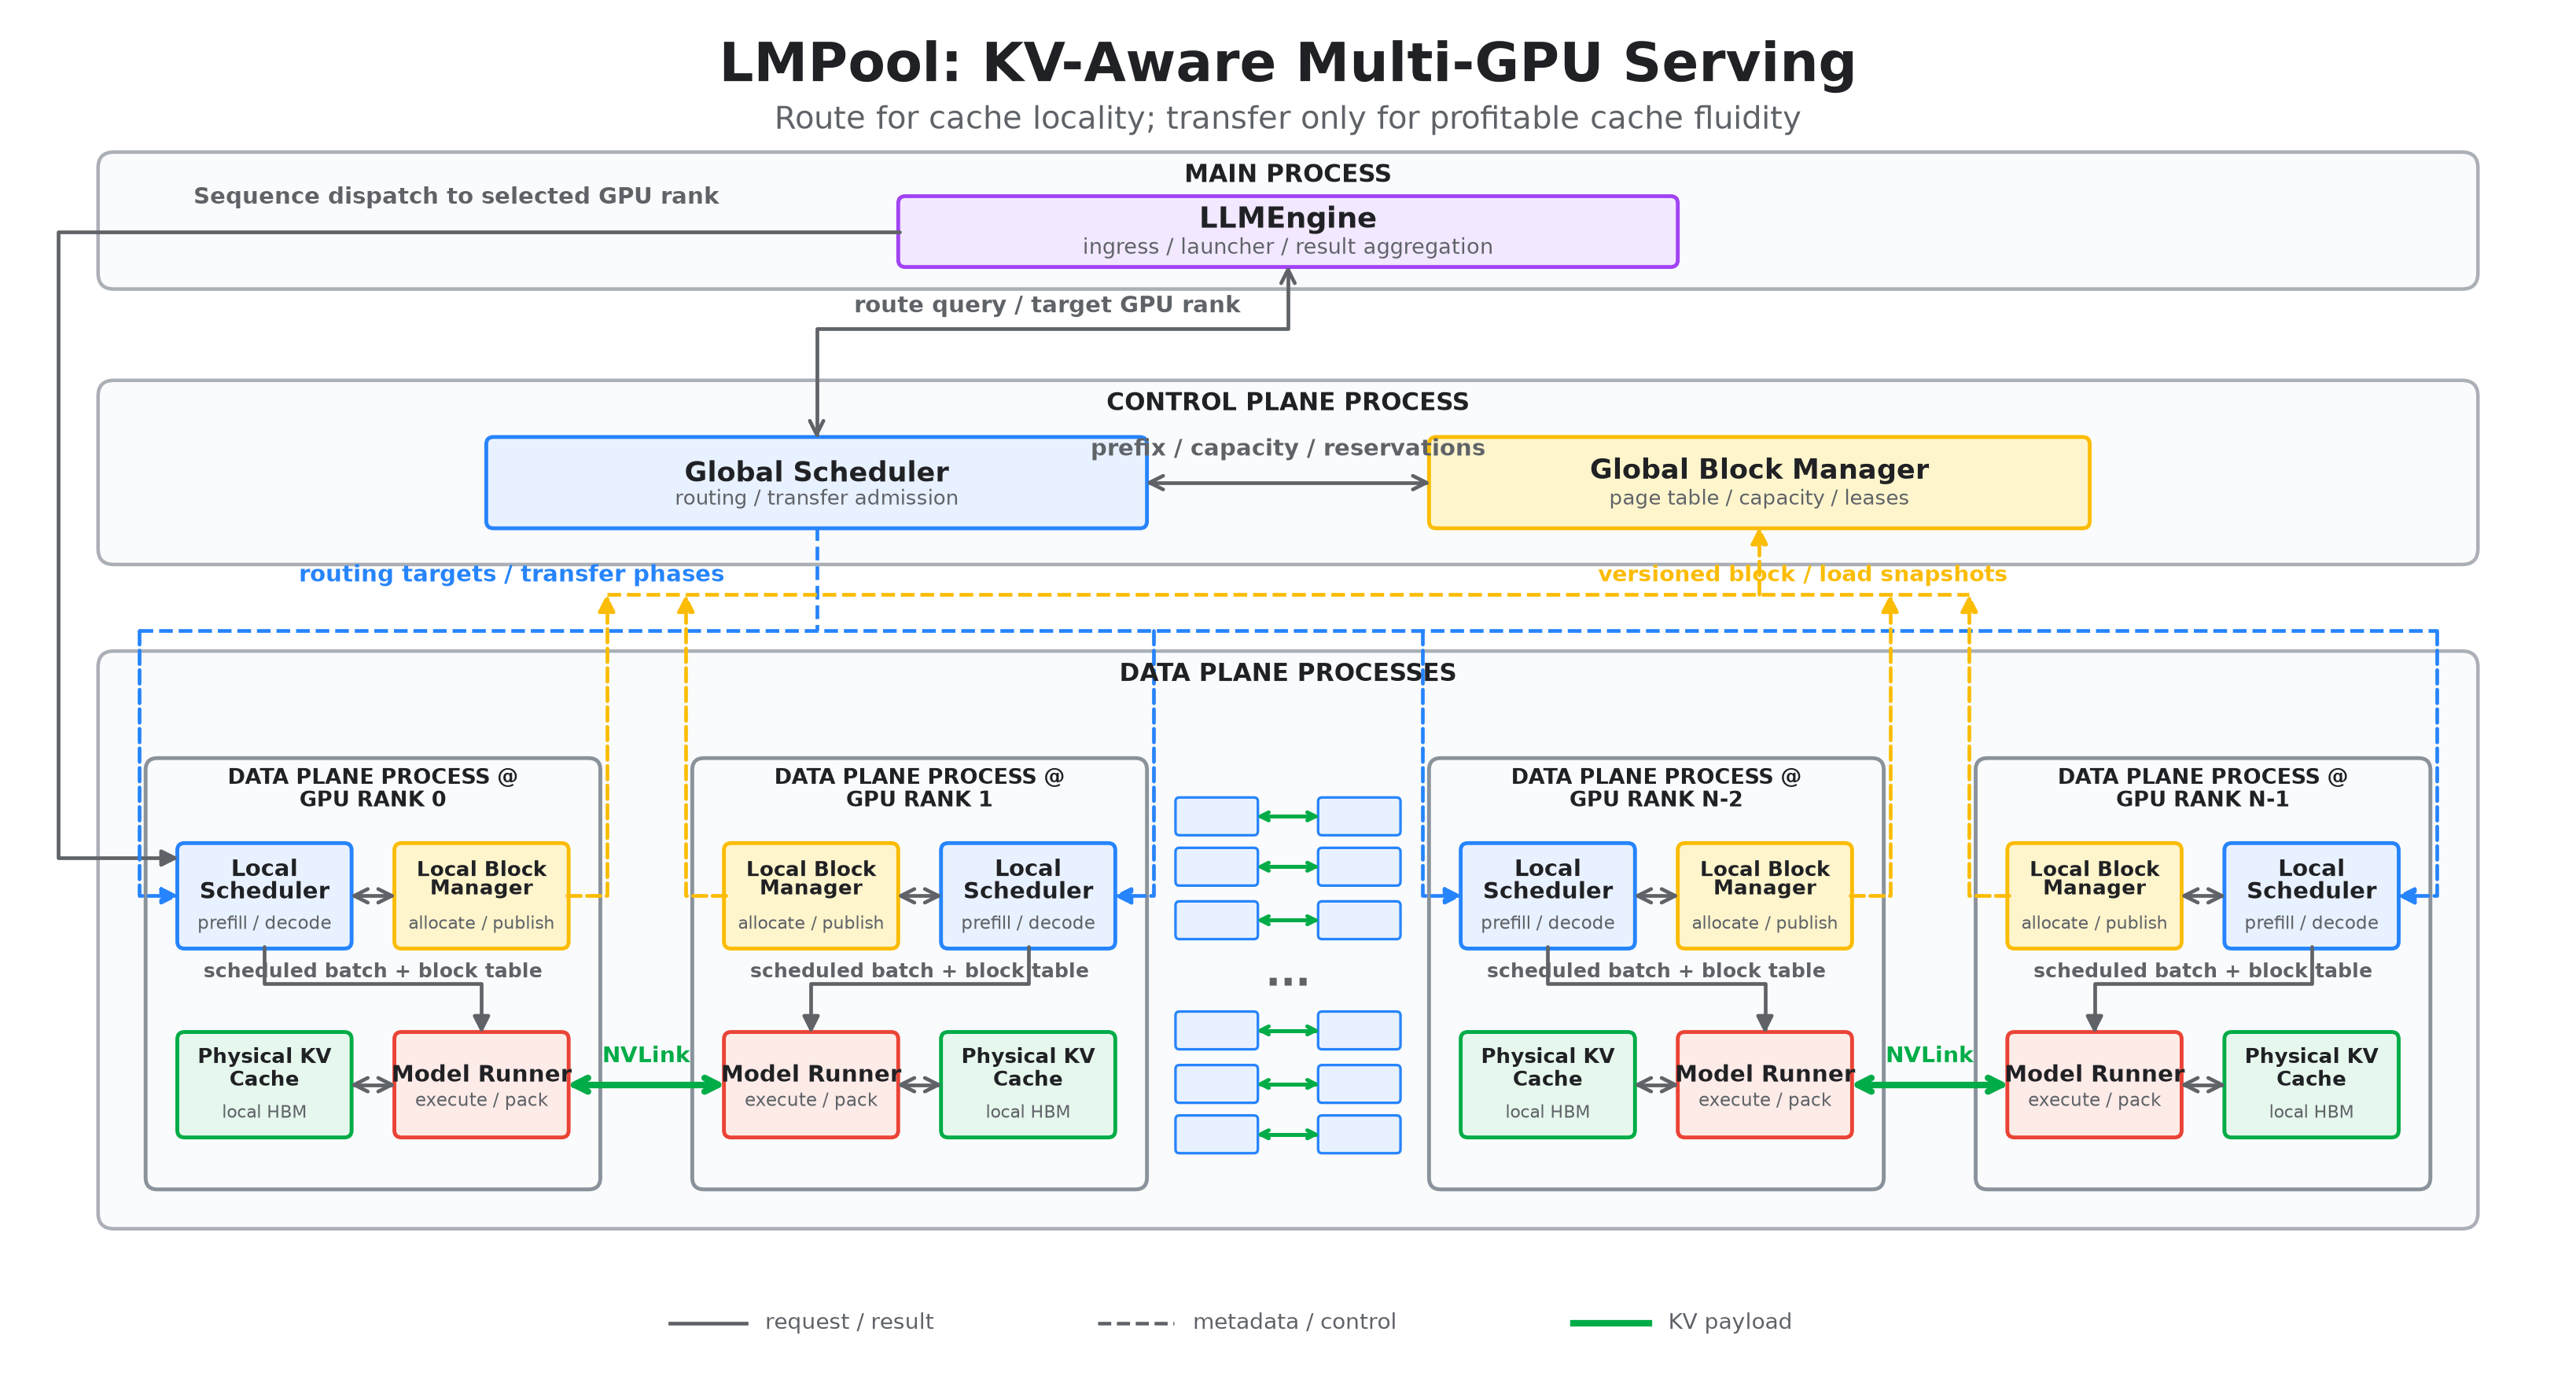
\includegraphics[width=0.92\textwidth]{fig_architecture.png}
  \caption{\sys{} 的 request、control、metadata 与 KV data path 分别位于 main process、
  control plane 和 per-GPU data plane。Global Scheduler 向每个 Local Scheduler 发送 routing 和
  transfer command；每个 Local Block Manager 向 Global Block Manager 发布版本化 block 与
  load snapshot。只有配对的 Model Runner 通过 NVLink path 交换打包 KV tensor，物理
  KV data 不经过 control plane。}
  \label{fig:arch}
\end{figure*}

图~\ref{fig:routing-decision}--\ref{fig:transfer-decision} 区分三个常被混淆的操作：
routing 选择请求执行的 GPU；background placement 预测需求并准入 candidate replica；
transactional transfer 验证并执行已准入 plan。图中的 decision node 展示 rejection、
deferral、spill 和 rollback path；hotness threshold 不能绕过 capacity、cooldown、
pair-idleness 或 measured-cost check。

\begin{figure*}[t]
  \centering
  
\includegraphics[width=0.9\textwidth]{fig_routing_decision.png}
  \caption{KV-aware routing 过滤不可行 GPU，并根据连续 prefix reuse、projected load 和
  capacity 选择 rank。仅当 prefix owner 的 load 足够高且额外 recomputation cost 受限时，
  bounded spill 才绕过 owner。}
  \label{fig:routing-decision}
\end{figure*}

\begin{figure*}[t]
  \centering
  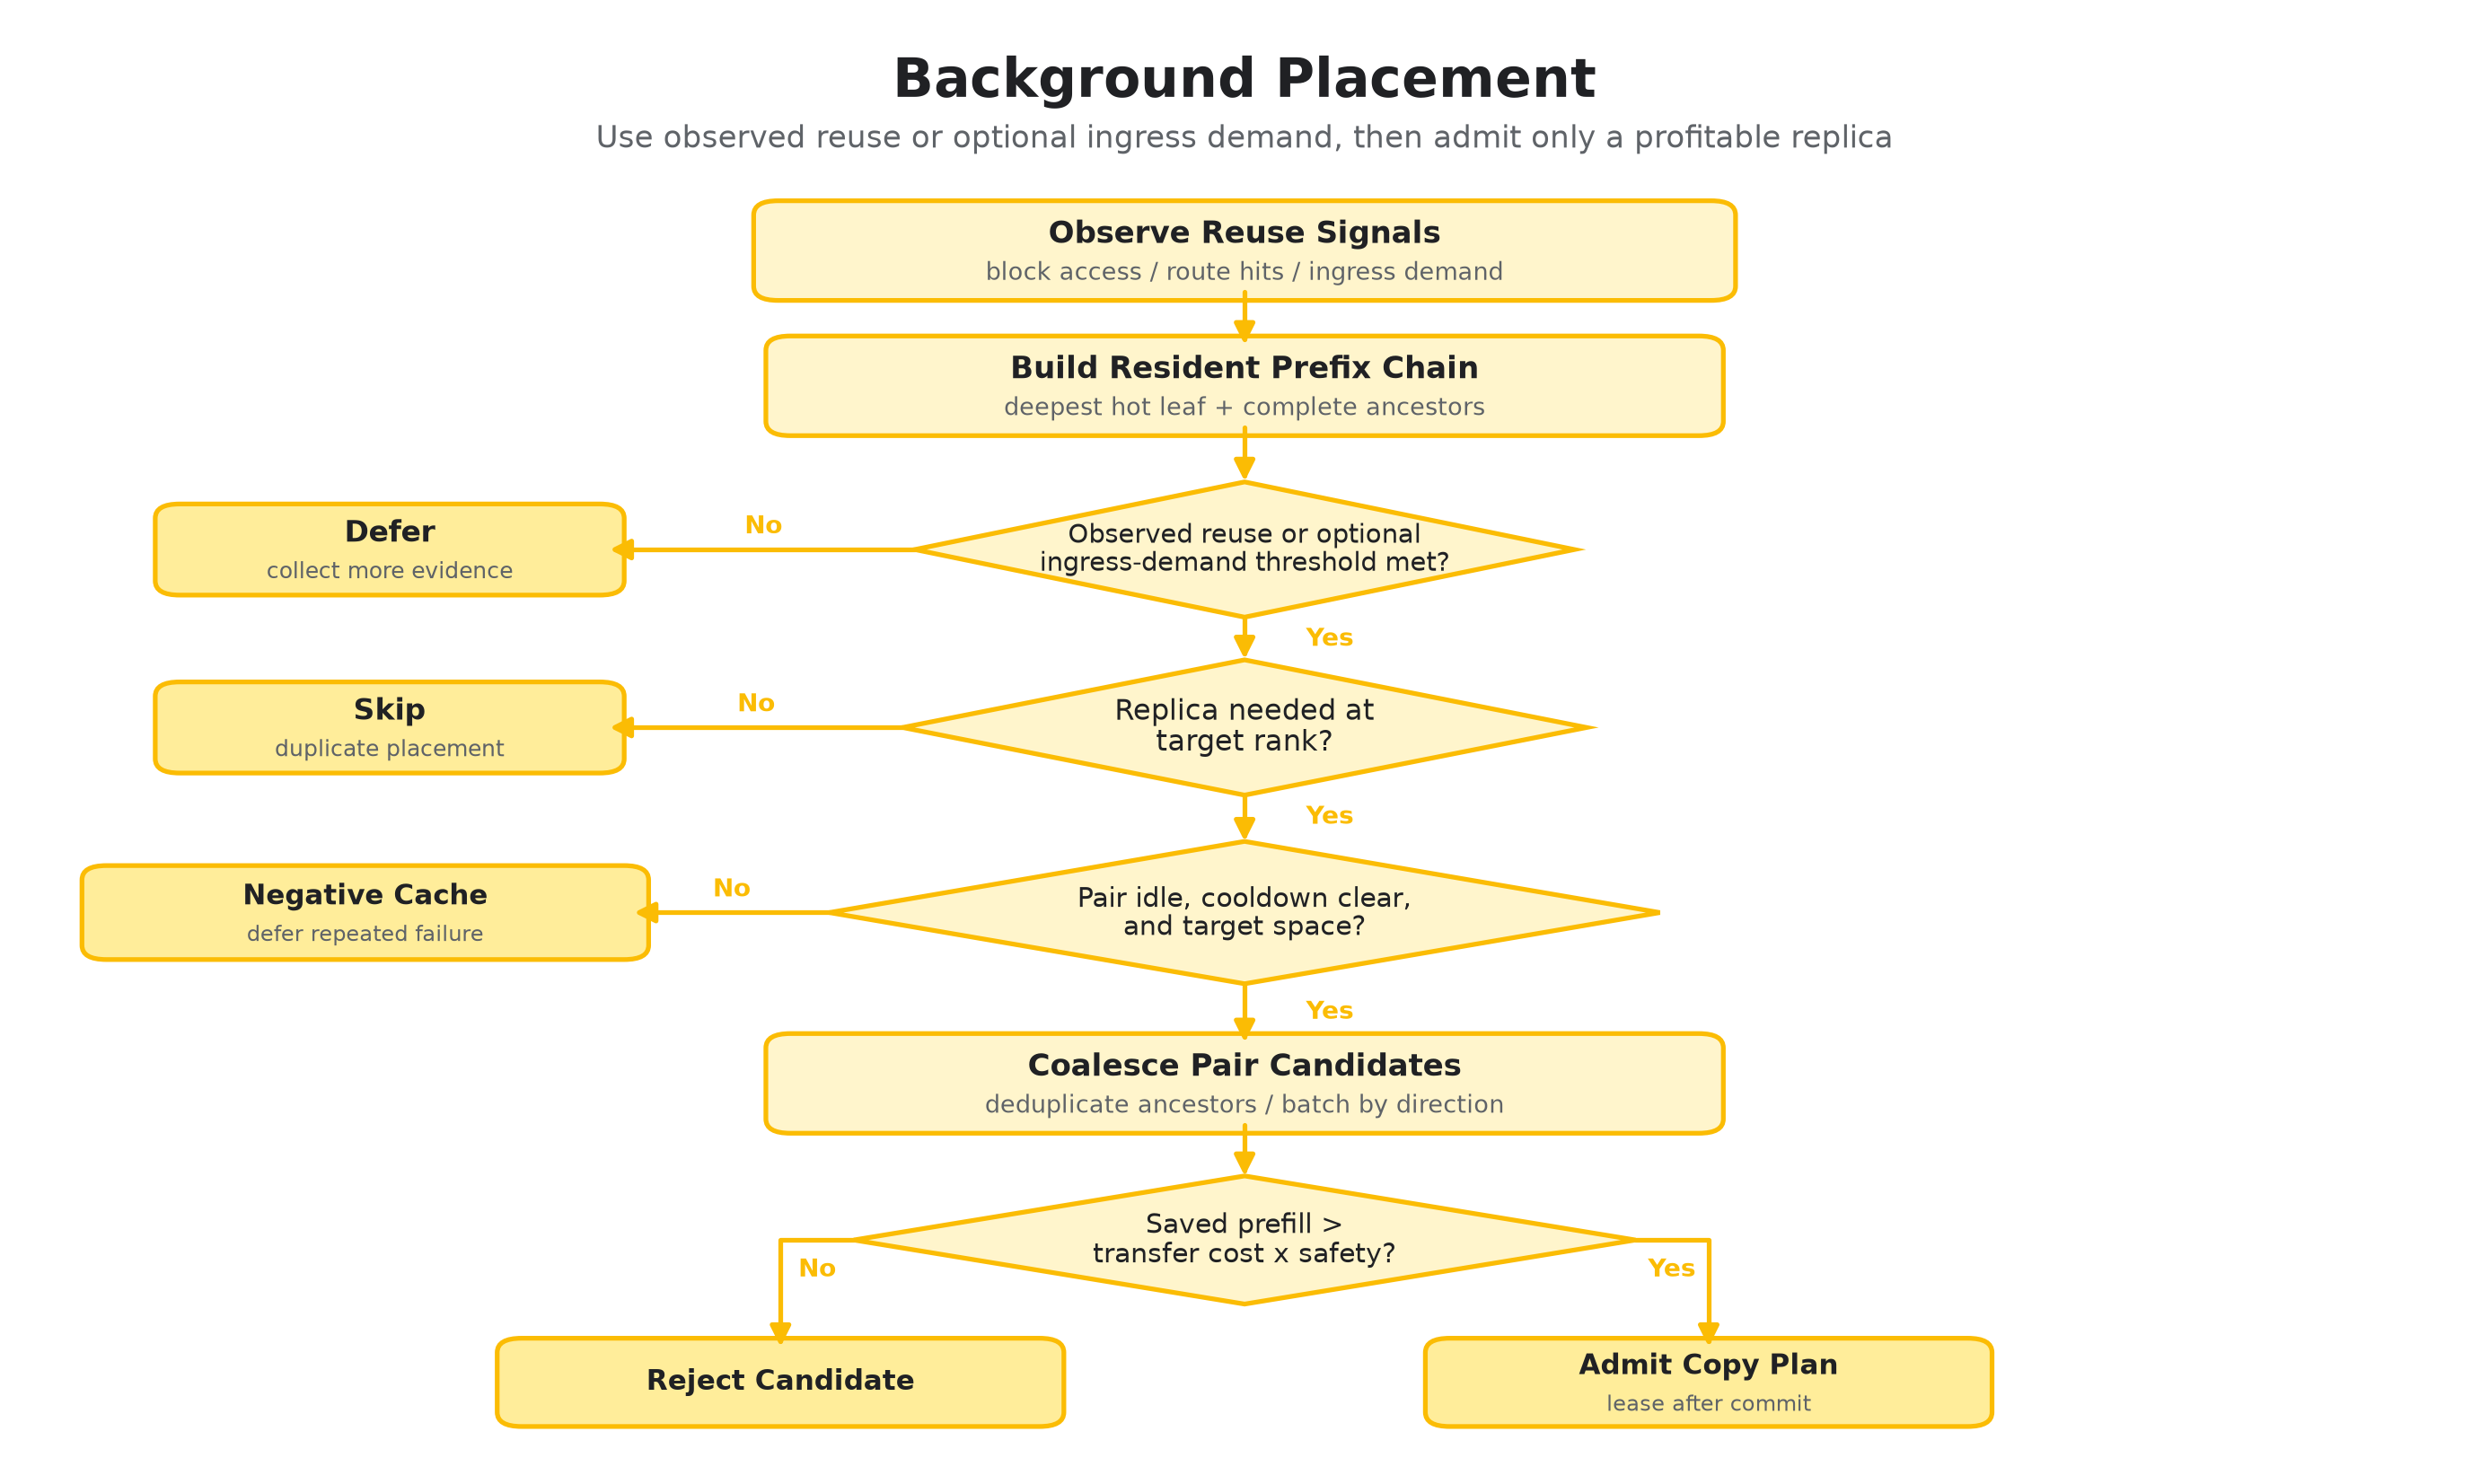
\includegraphics[width=0.9\textwidth]{fig_hot_prefix_decision.png}
  \caption{仅当 complete-block observation 或 ingress forecast 表示存在需求，且 cooldown、
  pair-idleness、target capacity 与 measured-benefit check 均通过时，background placement
  才准入 candidate replica。}
  \label{fig:hot-prefix-decision}
\end{figure*}

\begin{figure*}[t]
  \centering
  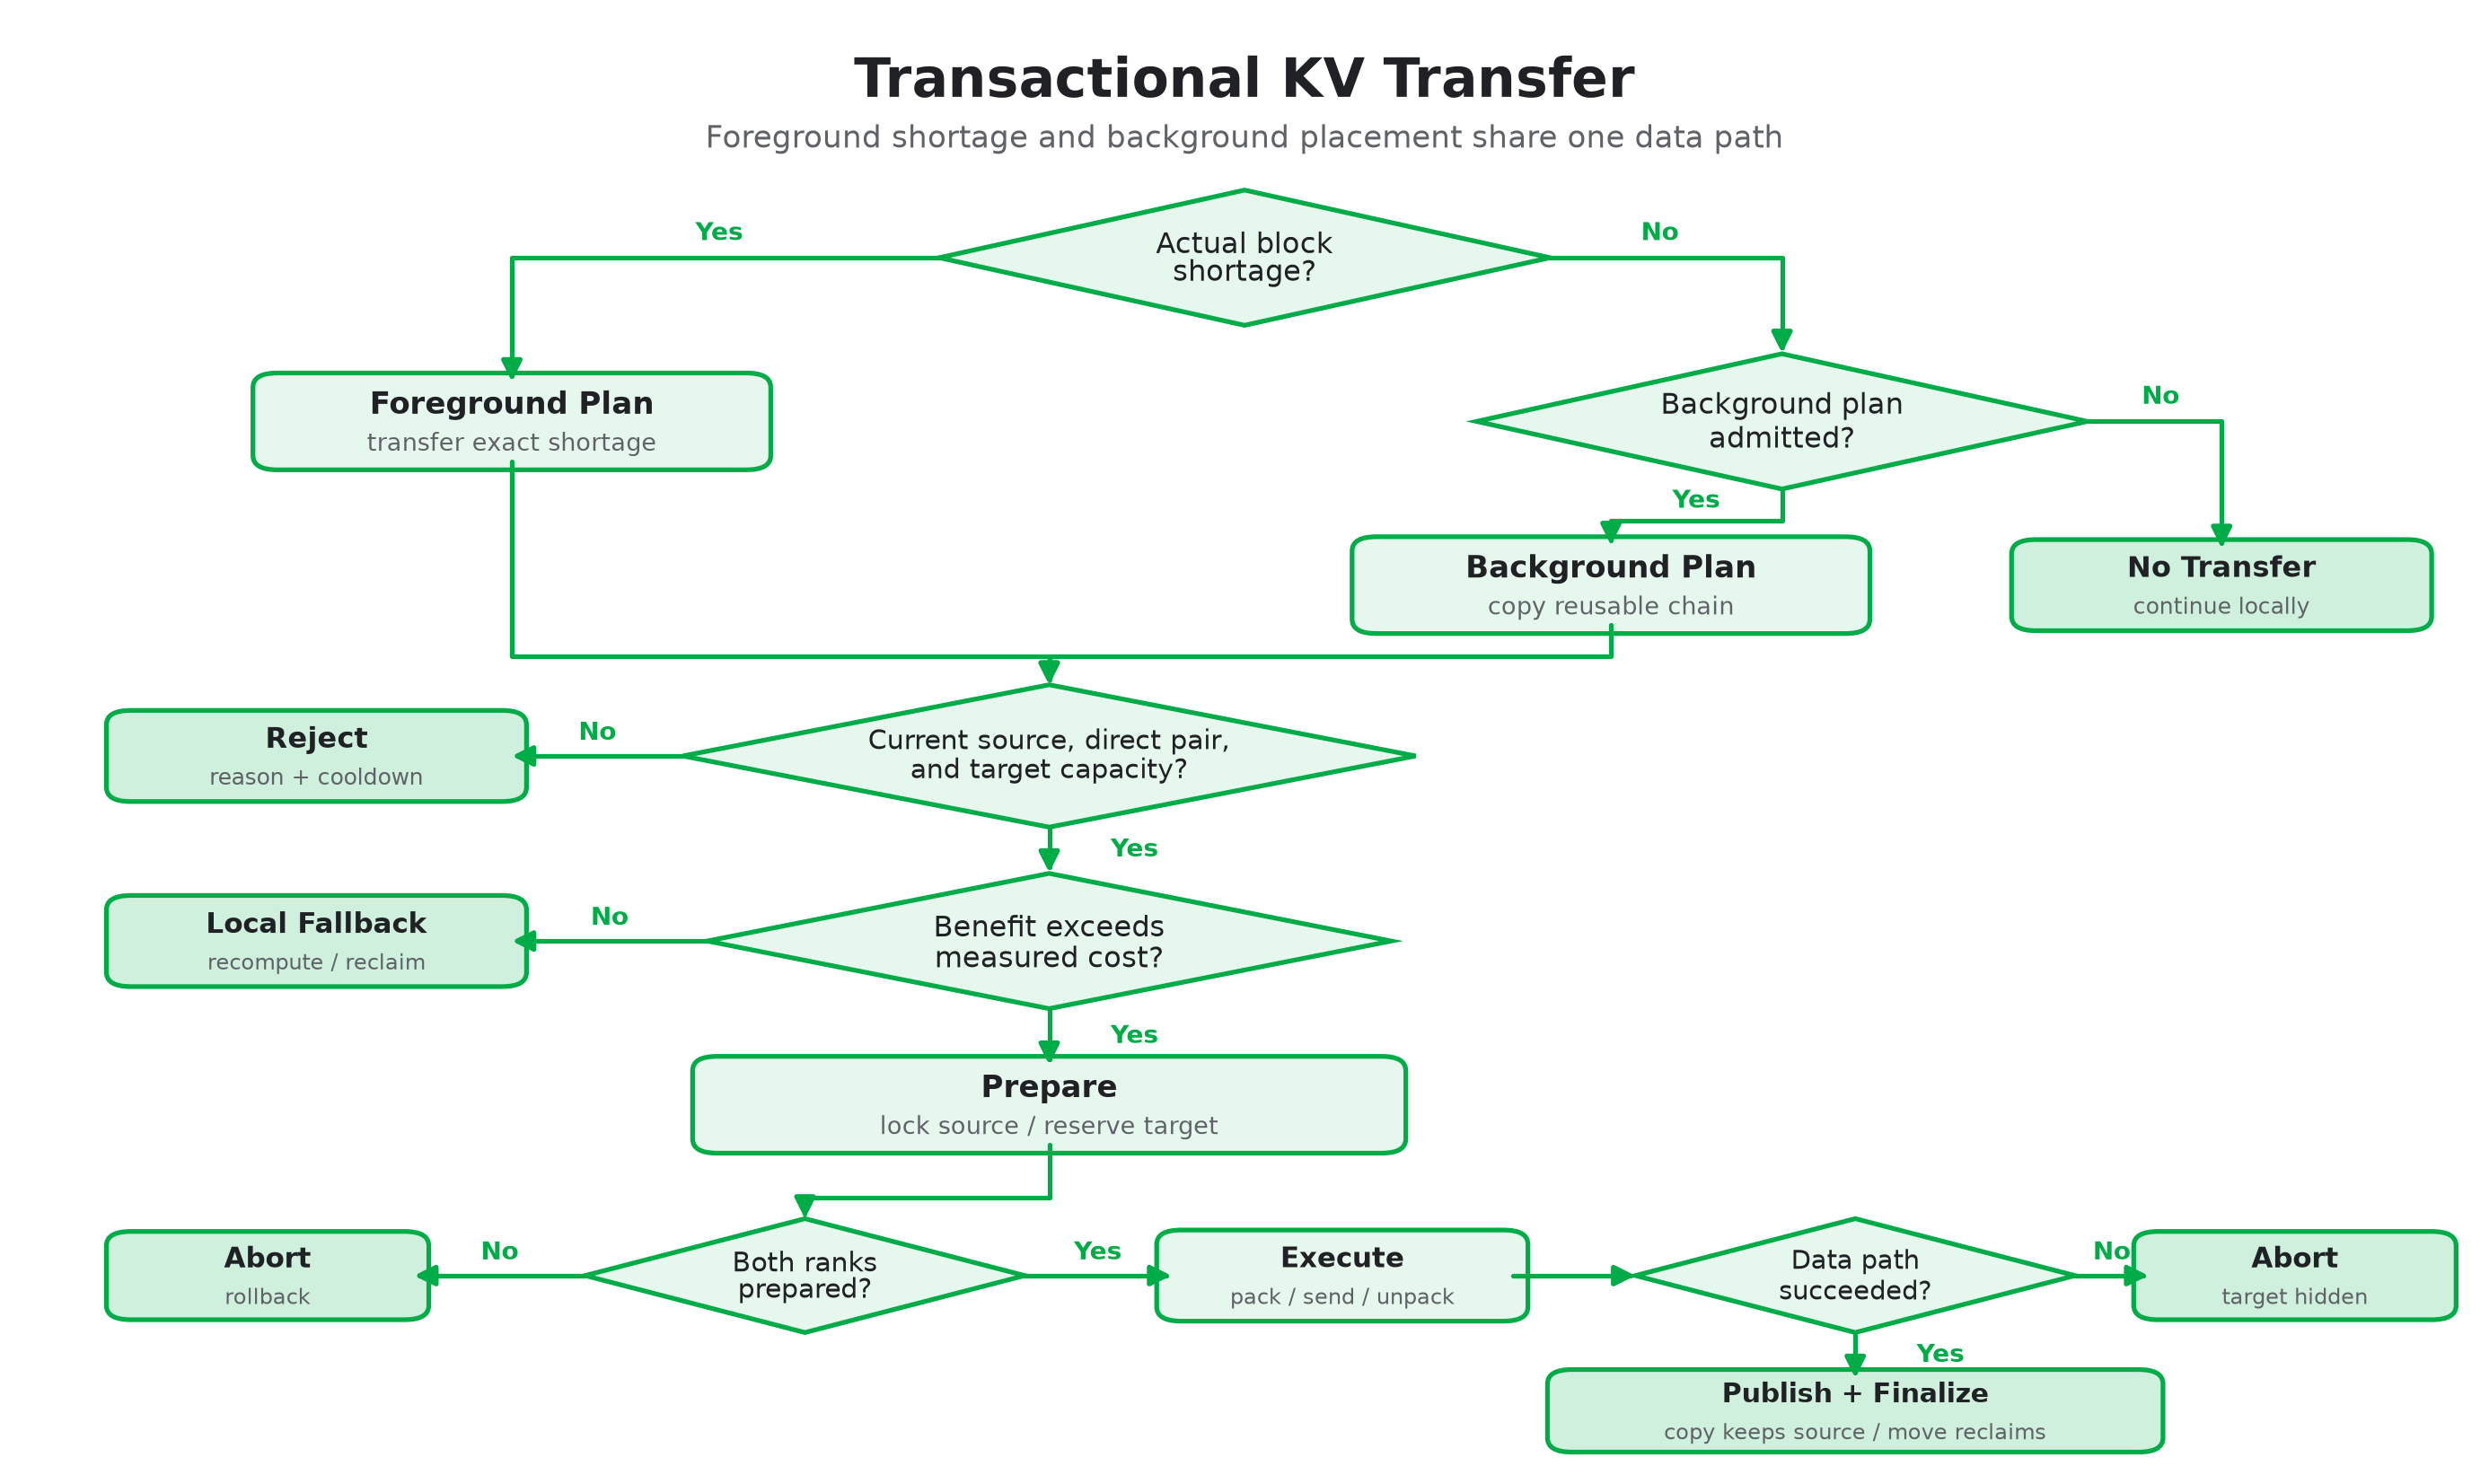
\includegraphics[width=0.9\textwidth]{fig_transfer_decision.png}
  \caption{Transactional transfer 对 foreground block shortage 或已准入 background chain
  依次执行 source validation、benefit check、preparation、pair-local NCCL transfer、
  publication 和 finalization。任一失败阶段均走 abort path，不暴露 destination。}
  \label{fig:transfer-decision}
\end{figure*}

\subsection{进程与所有权模型}

LLMEngine 是面向用户的进程。它启动一个独立 control-plane process 和 $N$ 个相同的
data-plane process，其中包括 rank~0 的 data-plane process。新 sequence 通过 LLMEngine
进入，后者经由 ControlPlaneClient 将 sequence metadata 与 prefix hash 发送给 control
plane。Control plane 在 LLMEngine 向选定 worker 入队完整 sequence 前选择 rank；worker
通常不会重复全局 routing。

Control process 拥有 GlobalScheduler 与 GlobalBlockManager。每个 data-plane process 拥有
一个 Local Scheduler、Local Block Manager、Model Runner 和 CUDA device。这一分离定义了
ownership boundary：global page table 是 global metadata 的 authoritative source，而每个
Local Block Manager 对 physical allocation、reference count、readiness 和 local KV tensor
具有 authoritative ownership。Global Scheduler 向每个 Local Scheduler 发送 routing target
与 transfer phase；每个 Local Block Manager 在相关 state change 后向 Global Block Manager
发送版本化 snapshot。

Request/result path 在 LLMEngine 和 selected worker 之间传递完整 Sequence object、generated
token 与 runtime measurement。Metadata/control path 向 control plane 传递版本化 block/load
snapshot，向 worker 传递 transfer phase 与 heartbeat command。KV data path 绕过 LLMEngine
和 control plane：source Model Runner 从 local HBM cache gather contiguous tensor，pair-local
NCCL communicator 通过 direct NVLink transfer，destination Model Runner 再将其 scatter 到
destination Local Block Manager 保留的 block。

LLMEngine 还会监控并可重启 control process。双向 heartbeat 检测无响应 worker 或 control
process，但不提供 consensus 或 high availability。control-process restart 后可由 worker state
snapshot 重建 control metadata；当前系统不能在 launcher failure 后继续服务。

\subsection{权威全局元数据}

GlobalBlockManager 维护 page table $h \mapsto \{(g,b,\mathrm{generation},\mathrm{ready})\}$，
可记录同一 hash 的多个 replica。对每张 GPU，它还保存 free、used、evictable block、parent
relationship、recency 与 access frequency 的版本化 snapshot。附加 state 包括 routing
reservation、active transfer 中的 block、placement lease、worker epoch 和用于拒绝 stale
update 的 snapshot version。

Worker 在 allocation、append、release、preemption、transfer publication 或相关 cache-access
change 后发布 complete snapshot。GlobalBlockManager 以单 GPU 为粒度原子替换 snapshot。
Routing 时产生的 reservation 会在 request commit 首次 prefill operation 前暂时减少可用容量，
防止一批 routing decision 重复消费同一 stale free-block count。Heartbeat reception 不推进
page-table freshness；缺失或 stale snapshot 会触发对 complete state 的显式请求。

\subsection{KV-Aware Routing}

LLMEngine 在将 ingress request 分配给 worker 前先提交给 GlobalScheduler。将该情形记为
$s=-1$，此时每个 healthy replica 都是 candidate，topology affinity $w(-1,g)=1$。对由
worker 发起、rank 为 $s\geq0$ 的 routing request，candidate set 包含 $s$ 及直接连接的
NVLink partner。令 $\mathcal{N}_{\mathrm{NV}}(s)$ 表示这些 partner，则
\begin{equation}
 w(s,g)=
 \begin{cases}
 2, & g=s,\\
 1, & g\in\mathcal{N}_{\mathrm{NV}}(s),\\
 0, & \text{其他情况}
 \end{cases}
\end{equation}
Affinity 为零的 candidate 在 cost evaluation 前被移除。该区分允许 global admission-time
routing，同时让 worker-originated rerouting 和 physical data movement 局限在已配置 direct pair。

对 candidate rank $g$，令 $N$ 为 prompt token 数，$R$ 为 request block 数，$h_g$ 为最长
contiguous ready-prefix match，$S$ 为 block size，$F_g$ 为当前 free block 数。所需新 block、
按 block 对齐的 uncached prefill work 与 reclamation pressure 为
\begin{align}
 n_g &= \max(0,R-h_g), & M_g &= \min(N,n_gS), & A_g &= \max(0,n_g-F_g).
\end{align}
只有 free capacity 与 dependency-safe reclaimable capacity 之和覆盖 $n_g$ 时，rank 才可行。
Token-equivalent queued work 为
\begin{equation}
\begin{aligned}
 Q_g ={}& w_w(T_g^{\mathrm{wait}}+T_g^{\mathrm{pending}})
          + w_rT_g^{\mathrm{running}} \\
        &+ w_s(N_g^{\mathrm{running}}+N_g^{\mathrm{pending}}),
\end{aligned}
\end{equation}
默认 $w_w=1$、$w_r=0.25$、$w_s=32$。GlobalScheduler 最小化
\begin{equation}
 C_{\mathrm{route}}(g) = Q_g + w_pM_g + w_eA_gS,
\end{equation}
默认 $w_p=1$、$w_e=0.5$。因此 locality 经由 $h_g$ 直接降低缺失 prefill work，而非作为从
cost 中扣除的独立 hit-rate reward；prefix 与 topology score 仅用于同成本 candidate 的 tie break。

\begin{figure*}[t]
  \centering
  
\includegraphics[width=0.96\textwidth]{fig_routing_cost_model.png}
  \caption{Routing cost 对每个 capacity-feasible rank 合并 token-aware queued work、
  block-rounded uncached prefill 与 dependency-safe reclamation pressure。仅当 prefix owner
  的 load 足够高、额外 recomputation cost 在配置限制内时允许 bounded spill。}
  \label{fig:routing-cost-model}
\end{figure*}

Router 选择 cost 最低的可行 candidate。当 owner 的 sequence pressure 比另一个 rank 高出
配置阈值且额外 recomputation cost 有界时，它可以绕过 prefix owner。当没有 candidate 含有
可复用 prefix 时，router 选择 projected cost 最低且 effective capacity 足够的 rank。该策略
缓解 request skew 和 replica underutilization，而不改变底层数据并行执行策略。

\subsection{本地分配与回收}

Local Block Manager 首先搜索匹配的 ready local block；命中后增加 reference count。若未命中，
它从 free deque 分配 block identifier，并只在 Model Runner 写入 KV data 后发布 complete block。
完成的 prefix 在 reference count 降至零后仍可 cache。Reclamation 仅考虑 dependency-safe leaf
block，避免移除 ancestor 导致保留 descendant 孤立。Replacement policy 结合 access frequency
与 recency。reference count 为正的 live block 不能作为 move-based eviction 的对象，但在
replication 有利时可被 copy。图~\ref{fig:kv-block-lifecycle} 概括 normal local path 和
transactional cross-GPU path。

\begin{figure*}[t]
  \centering
  
\includegraphics[width=0.98\textwidth]{fig_kv_block_lifecycle.png}
  \caption{KV block 在 Local Block Manager 所有权下经历 allocation、readiness、reference、
  caching、reservation、publication 和 reclamation state。Model Runner 写入或 transfer 物理
  K/V tensor；reserved 或 received 但未 published 的 block 对 routing 不可见。Publication
  先于 copy 或 move finalization；abort 保留 source 并释放 destination reservation。}
  \label{fig:kv-block-lifecycle}
\end{figure*}

``received'' 与 ``published'' 的区别定义了 visibility boundary。成功的 NCCL receive 本身不
创建可路由 replica；destination 必须先在 local snapshot 中记录 complete hash chain 与 readiness
state，之后 control plane 才可暴露新位置。Copy semantics 下，被引用的 source 保持有效，只会
被 unlock；move semantics 下，仅 unreferenced、dependency-safe suffix 可被 reclaim。partial 或
尚未 ready 的 local block 在 release 后绕过 cache，直接回到 free deque。

\subsection{Foreground Transfer}

Foreground transfer 由需求驱动。若 local prefill 或 decode append 期间出现 $k$ 个 block 的
shortage，worker 向 control plane 请求恰好 $k$ 个 block，而非该请求的完整 block count。
GlobalScheduler 选择 complete source chain 并决定操作为 move 或 copy。Publication 后，move
可在 source 释放 dependency-safe suffix，copy 则保留 source 并创建另一个 replica。Pinned
prefix 可以 copy，但不能释放。

对 $B$ 个 block、$L$ 个 layer、block size $S$、$H_{kv}$ 个 KV head、head dimension $D$ 与
每元素 $d$ byte，打包 payload 为 $X=2BLSH_{kv}Dd$。对每个 logical NVLink pair $p$，transfer
microbenchmark 提供单调 P95 data-path profile $\mathcal{P}_p=\{(X_i,Q^{95}_{p,i})\}$，另一
profile $\mathcal{R}_p=\{(X_i,R^{95}_{p,i})\}$ 记录已完成 serving transaction 的 P95 非负
dispatch-to-publication residual。Data-path prior 与 static estimate 为
\begin{align}
 T_{\mathrm{data}}^{p}(X) &= \operatorname{PWL}(X;\mathcal{P}_p), \\
 T_{\mathrm{static}}^{p}(X) &= \bigl(R^{95}_{p}(X)+I T_{\mathrm{data}}^{p}(X)\bigr)w_x.
\end{align}
模型在相邻 sample 间做线性插值；低于测量范围使用最近 boundary，高于范围则延伸最后一段
slope。令 $b(B)=2^{\lceil\log_2 B\rceil}$ 为 size bucket，已完成 source operation 和
dispatch-to-publication observation 分别更新非负 residual EWMA $\Delta^{src}_{p,b}$ 与
$\Delta^{place}_{p,b}$。Conservative admission estimate 为
\begin{equation}
\begin{aligned}
 T_{\mathrm{xfer}}=\max\bigl\{&T_{\mathrm{prior}}^{p},
 (T_{\mathrm{data}}^{p}+\Delta^{src}_{p,b})w_x,\\
 &(I T_{\mathrm{data}}^{p}+\Delta^{place}_{p,b})w_x\bigr\}.
\end{aligned}
\end{equation}
其中 $I=1.2$ 为 interference multiplier，$w_x$ 为配置的 transfer-cost weight。有 calibrated
residual profile 时 $T_{\mathrm{prior}}^{p}=T_{\mathrm{static}}^{p}$；无此 profile 时，先使用
zero-residual fallback，直至出现 completed placement observation，之后在 data-path estimate
与 online placement estimate 中取较大者。Residual profile 与 EWMA 均为非负，异常快 observation
不会使 admission 比 calibrated data-path prior 更激进。Foreground saved work 使用 discounted
historical chain reuse $\widehat{R}$；background admission 只计入第一次可避免的 cold prefill：
\begin{align}
 T_{\mathrm{save}}^{fg} &= \widehat{R}BS t_{\mathrm{prefill}}, &
 T_{\mathrm{save}}^{bg} &= BS t_{\mathrm{prefill}}(g_{dst}).
\end{align}
只有 source generation 与 target capacity 仍有效且 $T_{\mathrm{save}}\ge\rho T_{\mathrm{xfer}}$
时 plan 才被准入。具有相同 low-benefit 或 insufficient-capacity signature 的重复 background
candidate 会进入 negative cache，直到 signature 变化。

\begin{figure*}[t]
  \centering
  
\includegraphics[width=0.96\textwidth]{fig_transfer_cost_model.png}
  \caption{Transfer admission 将 expected saved prefill time 与相应 size bucket 的 pair-specific
  P95 latency profile 及 runtime residual 对比。Foreground 与 background path 对 saved work 的
  estimate 不同，但共享 validity、capacity 和 benefit-ratio check。}
  \label{fig:transfer-cost-model}
\end{figure*}

\subsection{Background Placement}

Background placement 解决可预测的未来 reuse，而不是即时 allocation failure。Worker 为 ready
block 报告 cumulative access count 与 parent hash。Control plane 按最深 hot leaf 选择 maximal
chain，并按 prefix order 重建所有 resident ancestor。Route-hit count 提供 online trigger；若
ingress 知道尚未提交的 queued request，也可提供从 hash 到 future demand 的 forecast。Forecast
可用时预测 reuse 受其上界限制；否则，预测 reuse 由 chain 上 minimum access count 减去 observed
use 并采用 conservative discount 得到。该信号只产生 candidate；admission 还要求 destination
不存在 replica、directed pair 的 cooldown 和 idle-pressure check 完成，且 target capacity 足够。

Compatible candidate 按 directed NVLink pair 去重并 batching。默认每个 candidate chain 至多
八个 block，每个 coalesced pair payload 至多 128 个 block；这只是上界，不是固定 transfer
size。Background admission 最多计入 destination 第一次可避免的 cold prefill，因为没有中间
eviction 时 destination 会在第一次 miss 后变 warm。Placement lease 只在 publication 后创建；
source 与 replica 的明确 quota 将后续 matching request 分配到两张 GPU，将 speculative placement
与 routing 耦合，而非仅复制数据。

Load-skew workload 在无 rank hint 情况下测试 background placement。Warm-up phase 为每个 hot
prefix 创建一个 instance，后续 burst 重用这些 prompt identity。Control plane 从 prefix ownership、
direct topology、capacity 和 load state 选择 source/target rank；placement lease 随后将完成的
replica 暴露给 routing。

\subsection{Transactional Transfer Protocol}

Transfer plan 有四个外部可见 phase。Preparation 中，destination reserve 具体 free block ID，
两个 worker 记录 plan state，routing 不能观察新位置。Execution 中，source/destination 发起
匹配的 NCCL point-to-point operation。Source 用 indexed selection 将 physical block gather 成
形状为 $[L,2,B,S,H_{kv},D]$ 的 contiguous tensor，分别表示 layer、K/V、transferred block、
block token、KV head 与 head dimension；预初始化的 pair-specific process group 一次 transfer
该 tensor。Destination receive 同形状 buffer，并用 indexed copy 将数据 scatter 到其 Local Block
Manager reserve 的 physical block。Hash、generation 和 destination block ID 是 control protocol
中的 metadata，不进入 NCCL tensor payload。

Publication 中，destination 将 received block 标为 ready 并发布 versioned snapshot；只有此后
control plane 才可暴露新的 page-table location 或 placement lease。Finalization 中，move 会在
释放指定 suffix 前验证每个 source block 的 hash 与 generation，copy 则保留 source。Preparation
或 execution 失败会 abort transaction、释放所有 reservation，并保留 source authority。

Protocol 对每个 plan ID 和 phase 都是 idempotent。Per-client receive lock 串行化 response queue
消费；一个 event loop 串行化 control-plane state mutation；每个 worker 内 block mutation 保持
single-threaded。这些措施保护 metadata transaction，同时不在 inference fast path 上引入 global
lock。

\section{实现}

\sys{} 使用 Python 与 PyTorch 扩展 Mini-vLLM。表~\ref{tab:modules} 总结了 implementation。

\begin{table}[t]
\centering\caption{主要实现模块}\label{tab:modules}\footnotesize
\setlength{\tabcolsep}{3.5pt}
\begin{tabular}{@{}L{0.30\linewidth}L{0.58\linewidth}@{}}\toprule
模块 & 职责\\\midrule
LLM engine & Request ingress、process launch/supervision、completion aggregation\\
Control plane & Protocol handling、client、authoritative event loop、heartbeat processing\\
Global scheduler & 基于 cost 的 routing 与 transfer-plan decision\\
Global block manager & Global page table、snapshot、reservation、candidate tracking\\
Data plane & Per-rank worker loop 与 transfer-phase execution\\
Local scheduler & Local prefill/decode admission 与 shortage detection\\
Local block manager & Physical block、prefix cache、reference 与 reclamation\\
Model runner & Model execution、KV tensor、metric 与 transfer interface\\
KV transfer & 打包 NCCL GPU-to-GPU payload movement\\\bottomrule
\end{tabular}\end{table}

\subsection{测试策略}

我为每个 engine module 实施了 unit test。表~\ref{tab:tests} 总结 coverage。
测试使用 fake component 获得 deterministic control decision。

\begin{table}[t]
\centering\caption{测试设计与覆盖范围}\label{tab:tests}\footnotesize
\setlength{\tabcolsep}{3.5pt}
\begin{tabular}{@{}p{0.28\linewidth}p{0.58\linewidth}@{}}\toprule
测试组 & 覆盖行为\\\midrule
Block manager & Allocation/release、chain reuse、LFU/LRU leaf、generation、snapshot\\
Global scheduler & Hit/miss/capacity route、load bypass、direct-pair filter、move/copy plan\\
Control plane & Epoch、stale update、reservation、lease、idempotent phase、heartbeat、concurrency\\
Data plane/engine & Queue protocol、master-first ingress、worker/control lifecycle、result aggregation\\
KV transfer & Shape/byte accounting、copy/move primitive、two-rank NCCL equality、deadlock detection\\
Model runner & KV layout、prefill/decode preparation、dtype consistency、transfer adapter\\
Benchmark & Workload、schema、metric、confidence interval、plotting、profile construction/validation\\
End-to-end & Multi-process completion 与 optional CUDA/NCCL integration\\\bottomrule
\end{tabular}\end{table}

\section{评估}

评估回答四个问题：(Q1) KV-aware routing 是否在长共享前缀下改善有效 prefix reuse 和 service？
(Q2) Transfer data path 提供何种 latency/bandwidth？(Q3) Background copy 与 placement lease 是否
在 load skew 下执行，它们带来什么 serving trade-off？(Q4) Foreground move 是否能在 memory skew
下安全释放 source capacity？Q1 是主要端到端性能主张；Q2--Q4 证明 data-path correctness、protocol
behavior 与 completed transfer 不产生增量服务收益的边界。

\subsection{设置与方法}

评估在一台七 GPU host 中选取六张 24~GiB GeForce RTX 3090。实测 topology 有三组 direct pair：
physical GPU $(0,1)$、$(3,4)$ 和 $(5,6)$；benchmark 将其分别暴露为 logical pair $(0,1)$、
$(2,3)$、$(4,5)$。NVLink topology 与 peer-access matrix 均显示每个 selected pair 内为 direct
path、pair 间无 direct path。NV4 表示四条 bonded link。RTX 3090
使用 GA102 的 third-generation NVLink interface；每条 link 单向 14.0625~GB/s，因此一组 four-link
pair 理论单向峰值为 56.25~GB/s，双向合计 112.5~GB/s~\citep{NVIDIAAmpereGA102}。KV-transfer
workload 是单向的，因此与 56.25~GB/s 上限比较。

使用 BF16 的 Qwen3-0.6B 与 Qwen3-1.7B；两者均有 28 layer、八个 KV head 和 128 head dimension，
即每 token 114,688 KV byte。KV block size 为 256 token。每个 system experiment 使用每 worker 固定
KV block budget，以 seed~0 重复五次，禁用 EOS termination。Routing、memory skew、load skew 分别
生成 64、16、8 个 output token；goodput 使用 workload-specific E2E SLA。每个 JSON artifact 记录
command、resolved model configuration、Git state、individual trial value、95\% confidence interval 与
per-rank statistic。每个 scenario 在 fresh process 中运行，cache content 不跨 scenario 保留；完整
artifact 对应结果 `20260727T231622Z`。

\subsection{合成数据集剖析}

研究使用 deterministic synthetic prompt，而非 public conversational trace。每个 prompt 将 Qwen chat
template 应用于 repeated instruction body 和 group-specific suffix，使可复用 KV state 的数量与 ownership
显式可控。表~\ref{tab:datasets} 对 tokenized input 与 phase structure 进行 profiling；仅有 request
hit rate 不足以量化可复用 prompt token。

在应用任何 system policy 前，报告两个 intrinsic trace metric。令 $m_i$ 为请求 $i$ 中 cumulative
hash 已出现在先前请求、且连续完整的 prefix block 数，$B$ 为 block size，$T_i$ 为 prompt length。
Request prefix sharing 为 $\sum_i\mathbb{1}[m_i>0]/N$，token prefix sharing 为
$B\sum_i m_i/\sum_i T_i$。这些数值是 unlimited cache capacity 与 perfect placement 下的 ordered-replay
upper bound，且不含 partial tail block；runtime request hit 与 cached-token ratio 另行报告。

\begin{table}[!htbp]\centering\caption{合成工作负载剖析}\label{tab:datasets}\scriptsize
\setlength{\tabcolsep}{1.5pt}\renewcommand{\arraystretch}{1.08}
\begin{tabularx}{\linewidth}{@{}L{0.07\linewidth}L{0.05\linewidth}Y L{0.10\linewidth}L{0.07\linewidth}L{0.10\linewidth}L{0.05\linewidth}Y@{}}\toprule
工作负载 & 请求数 & 前缀构造 & Prompt token & 请求共享 & Token 共享 & Window & 目的\\\midrule
Routing & 192 & 16 个 recurring group；每组首请求为 cold；共享前缀长度为 1x、3x、5x & 365,880 / 1,084,728 / 1,803,576 & 91.67\% & 86.20\% / 91.38\% / 89.93\% & 16 & 隔离 locality-aware routing。\\
Load skew & 192 & 三个长 hot group；三个 warm-up 后为 189 次 hot reuse & 1,444,344 & 98.44\% & 97.15\% & 96 & 测试 background copy 与 placement lease。\\
Memory skew & 72 & 六个 session warm-up、30 个 anchor/cold pressure request、36 个 session reuse & 486,554 & 91.67\% & 72.29\% & 48 & 测试 move-style source-capacity release。\\\bottomrule
\end{tabularx}\end{table}

\subsection{Baseline 与指标}

定义五个 normalized scenario：single-gpu 运行一个 replica；multi-gpu 使用 static round-robin data
parallelism；multi-gpu-kv-routing 开启 global routing、关闭 transfer；multi-gpu-kv-transfer 保持
round-robin request placement、开启 transfer；multi-gpu-lmpool 同时开启两种机制。所有 multi-GPU
scenario 每 worker 使用相同 KV block budget。这些 scenario 是受控内部消融，隔离 routing/transfer
的增量作用，并保持 model execution、KV capacity 与 request generation 不变；它们不是与 production
vLLM、SGLang、Mooncake 或 LMCache deployment 的直接比较。

主要指标为 output throughput、SLA goodput、mean TTFT、decode time per output token (TPOT)、mean/P90
E2E latency 和 uncached prefill token。对请求 $i$，令 $s_i$ 为 submission time、$f_i$ 为 first-token
time、$c_i$ 为 completion time、$N_i$ 为 output token 数，则 $\mathrm{TTFT}_i=f_i-s_i$，
$\mathrm{TPOT}_i=(c_i-f_i)/(N_i-1)$。$N_i=1$ 的请求无 decode interval，不计入 TPOT statistic。
该定义排除 queueing/prefill time。另报告 control-plane request hit、route-to-owner hit、data-plane
local request hit 与 cached-token ratio。Transfer counter 报告 block/payload byte、copy/move operation、
protocol outcome、estimated/observed cost；per-rank request、token、execution time 和 utilization 分布
揭示 load concentration。

对 $R$ 次完整重复测得的 metric，报告 sample mean
$\bar{x}=R^{-1}\sum_{r=1}^{R}x_r$ 与双侧 95\% confidence interval
$\bar{x}\pm t_{0.975,R-1}s/\sqrt{R}$，其中 $s$ 为 sample standard deviation。实验 $R=5$，
$t_{0.975,4}=2.776$。对 P90 E2E 等 tail metric，$x_r$ 是第 $r$ 次重复中的 request-level P90，
区间则在五个 repetition-level P90 间计算。这些区间量化固定设置下 run-to-run variation，而非
request-level latency distribution 或 model/hardware 间变化。

\begin{figure*}[t]\centering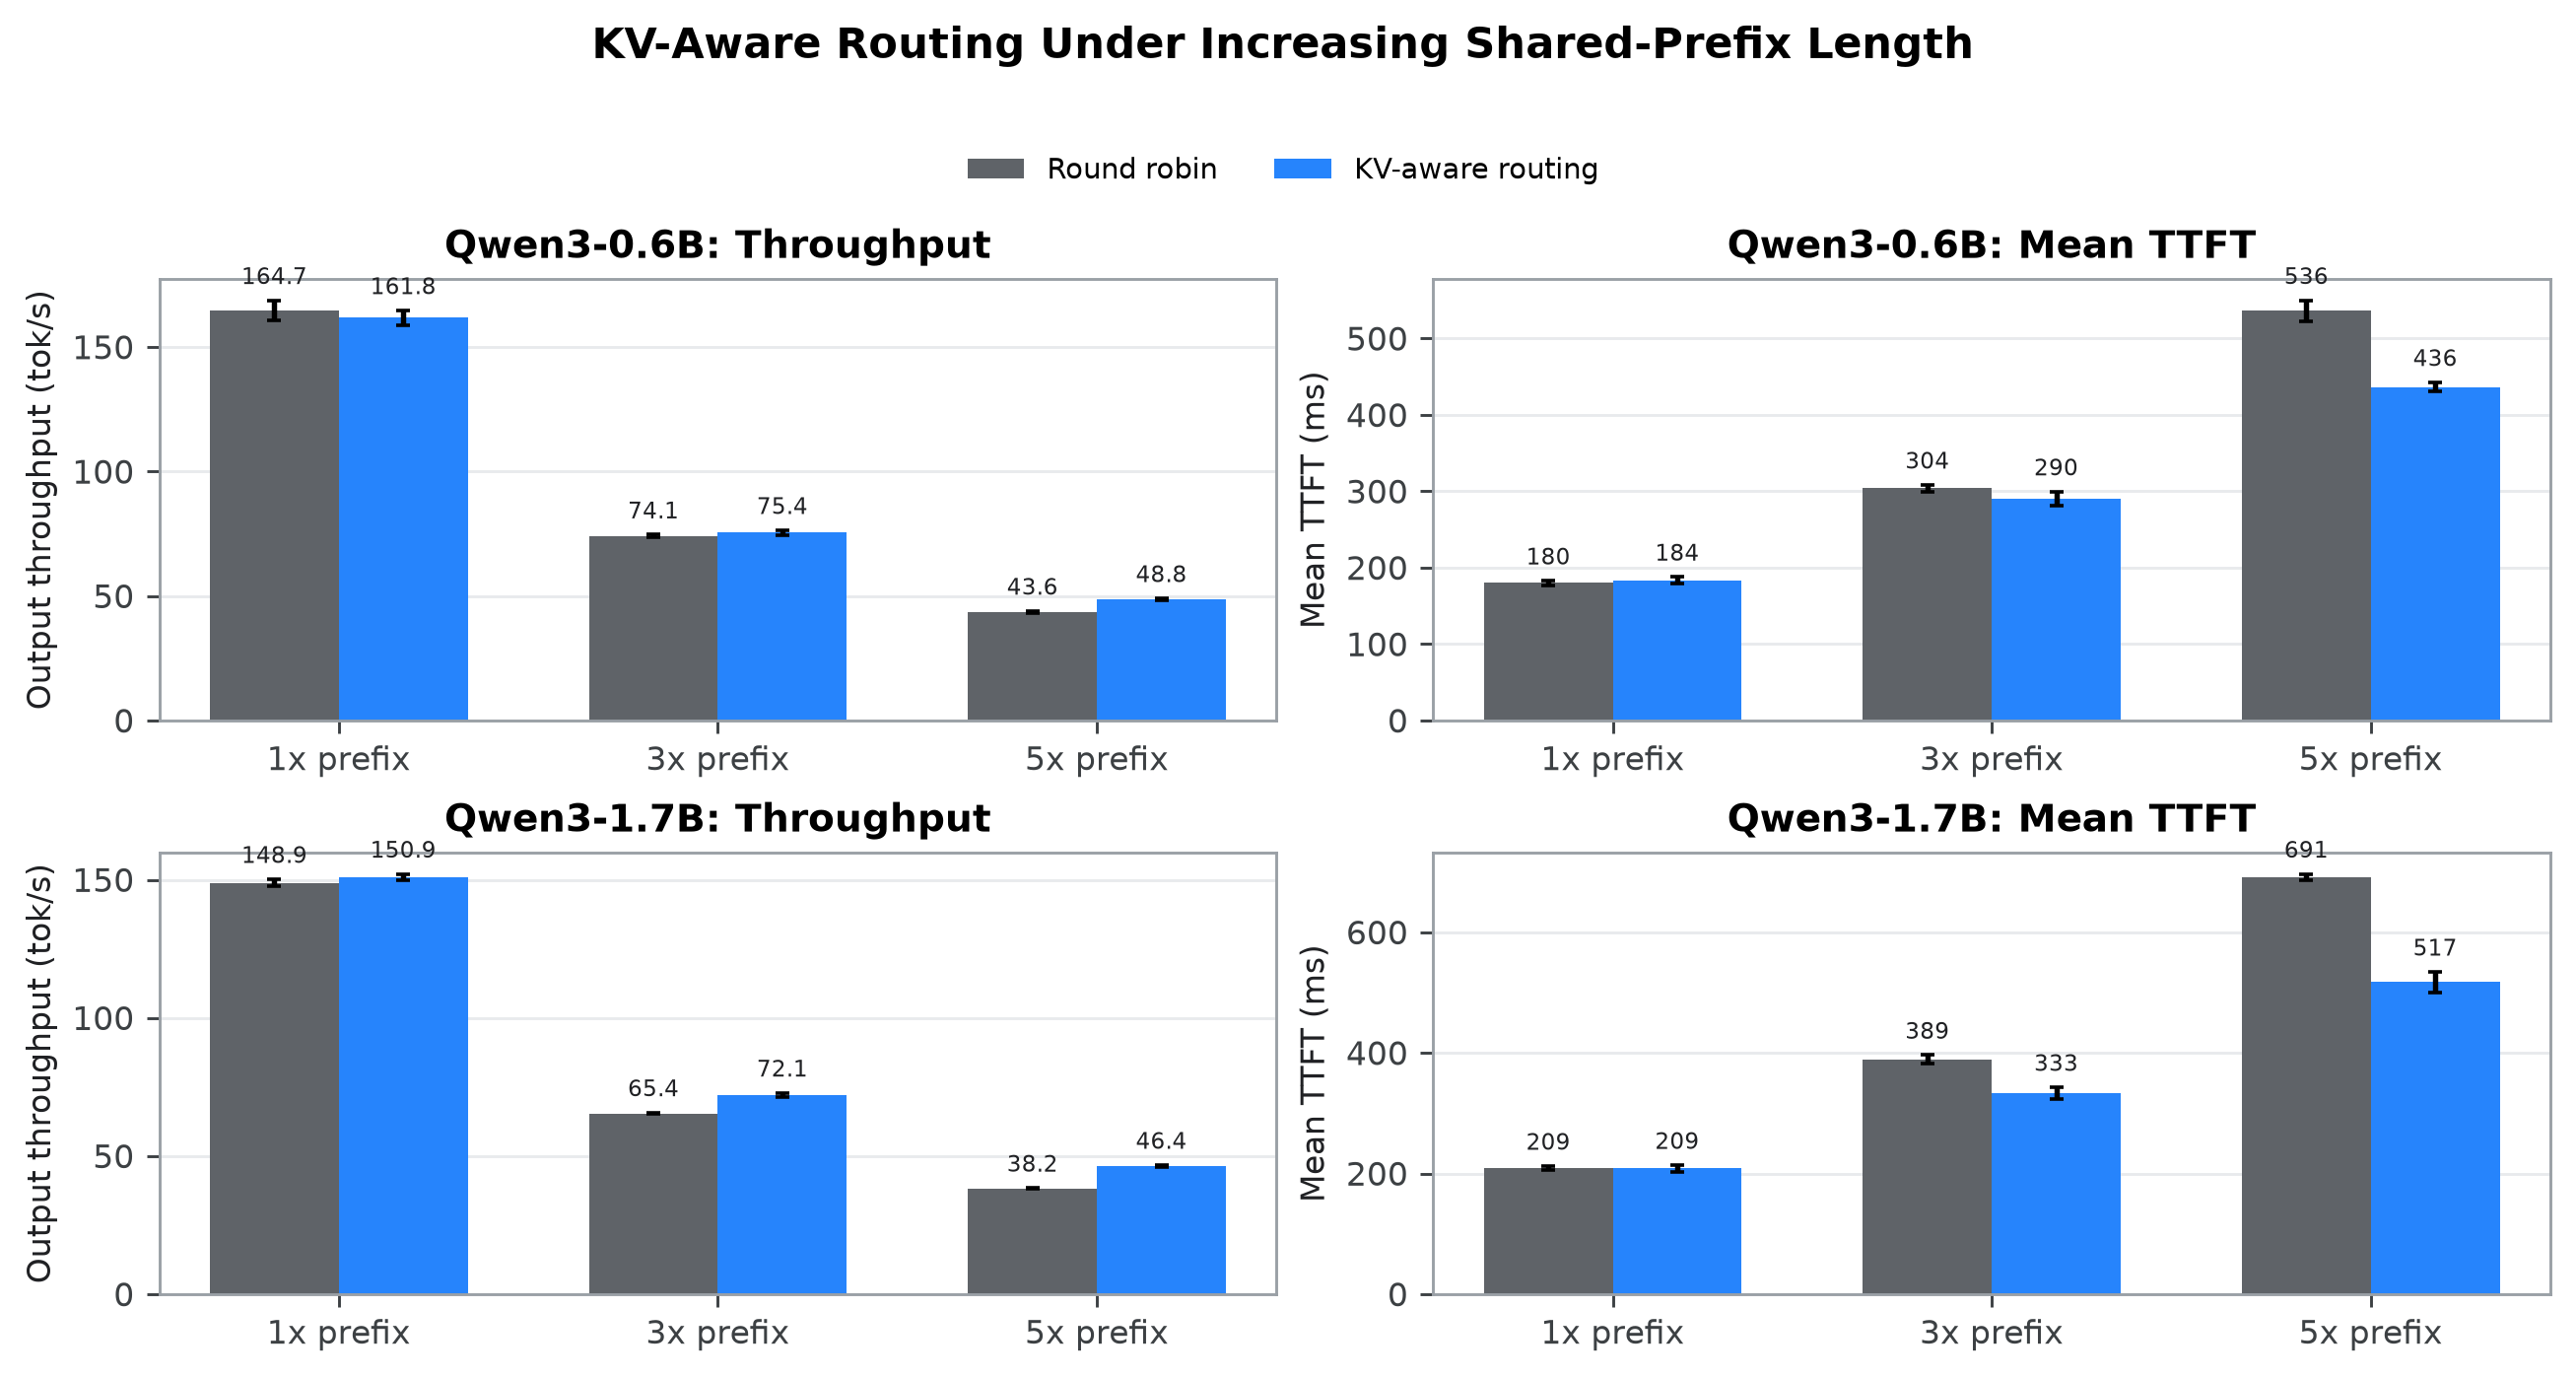
\includegraphics[width=\textwidth]{fig_suite_routing.png}
\caption{随共享前缀长度增加的 Routing 结果}\label{fig:suite-routing}\end{figure*}
\begin{figure*}[t]\centering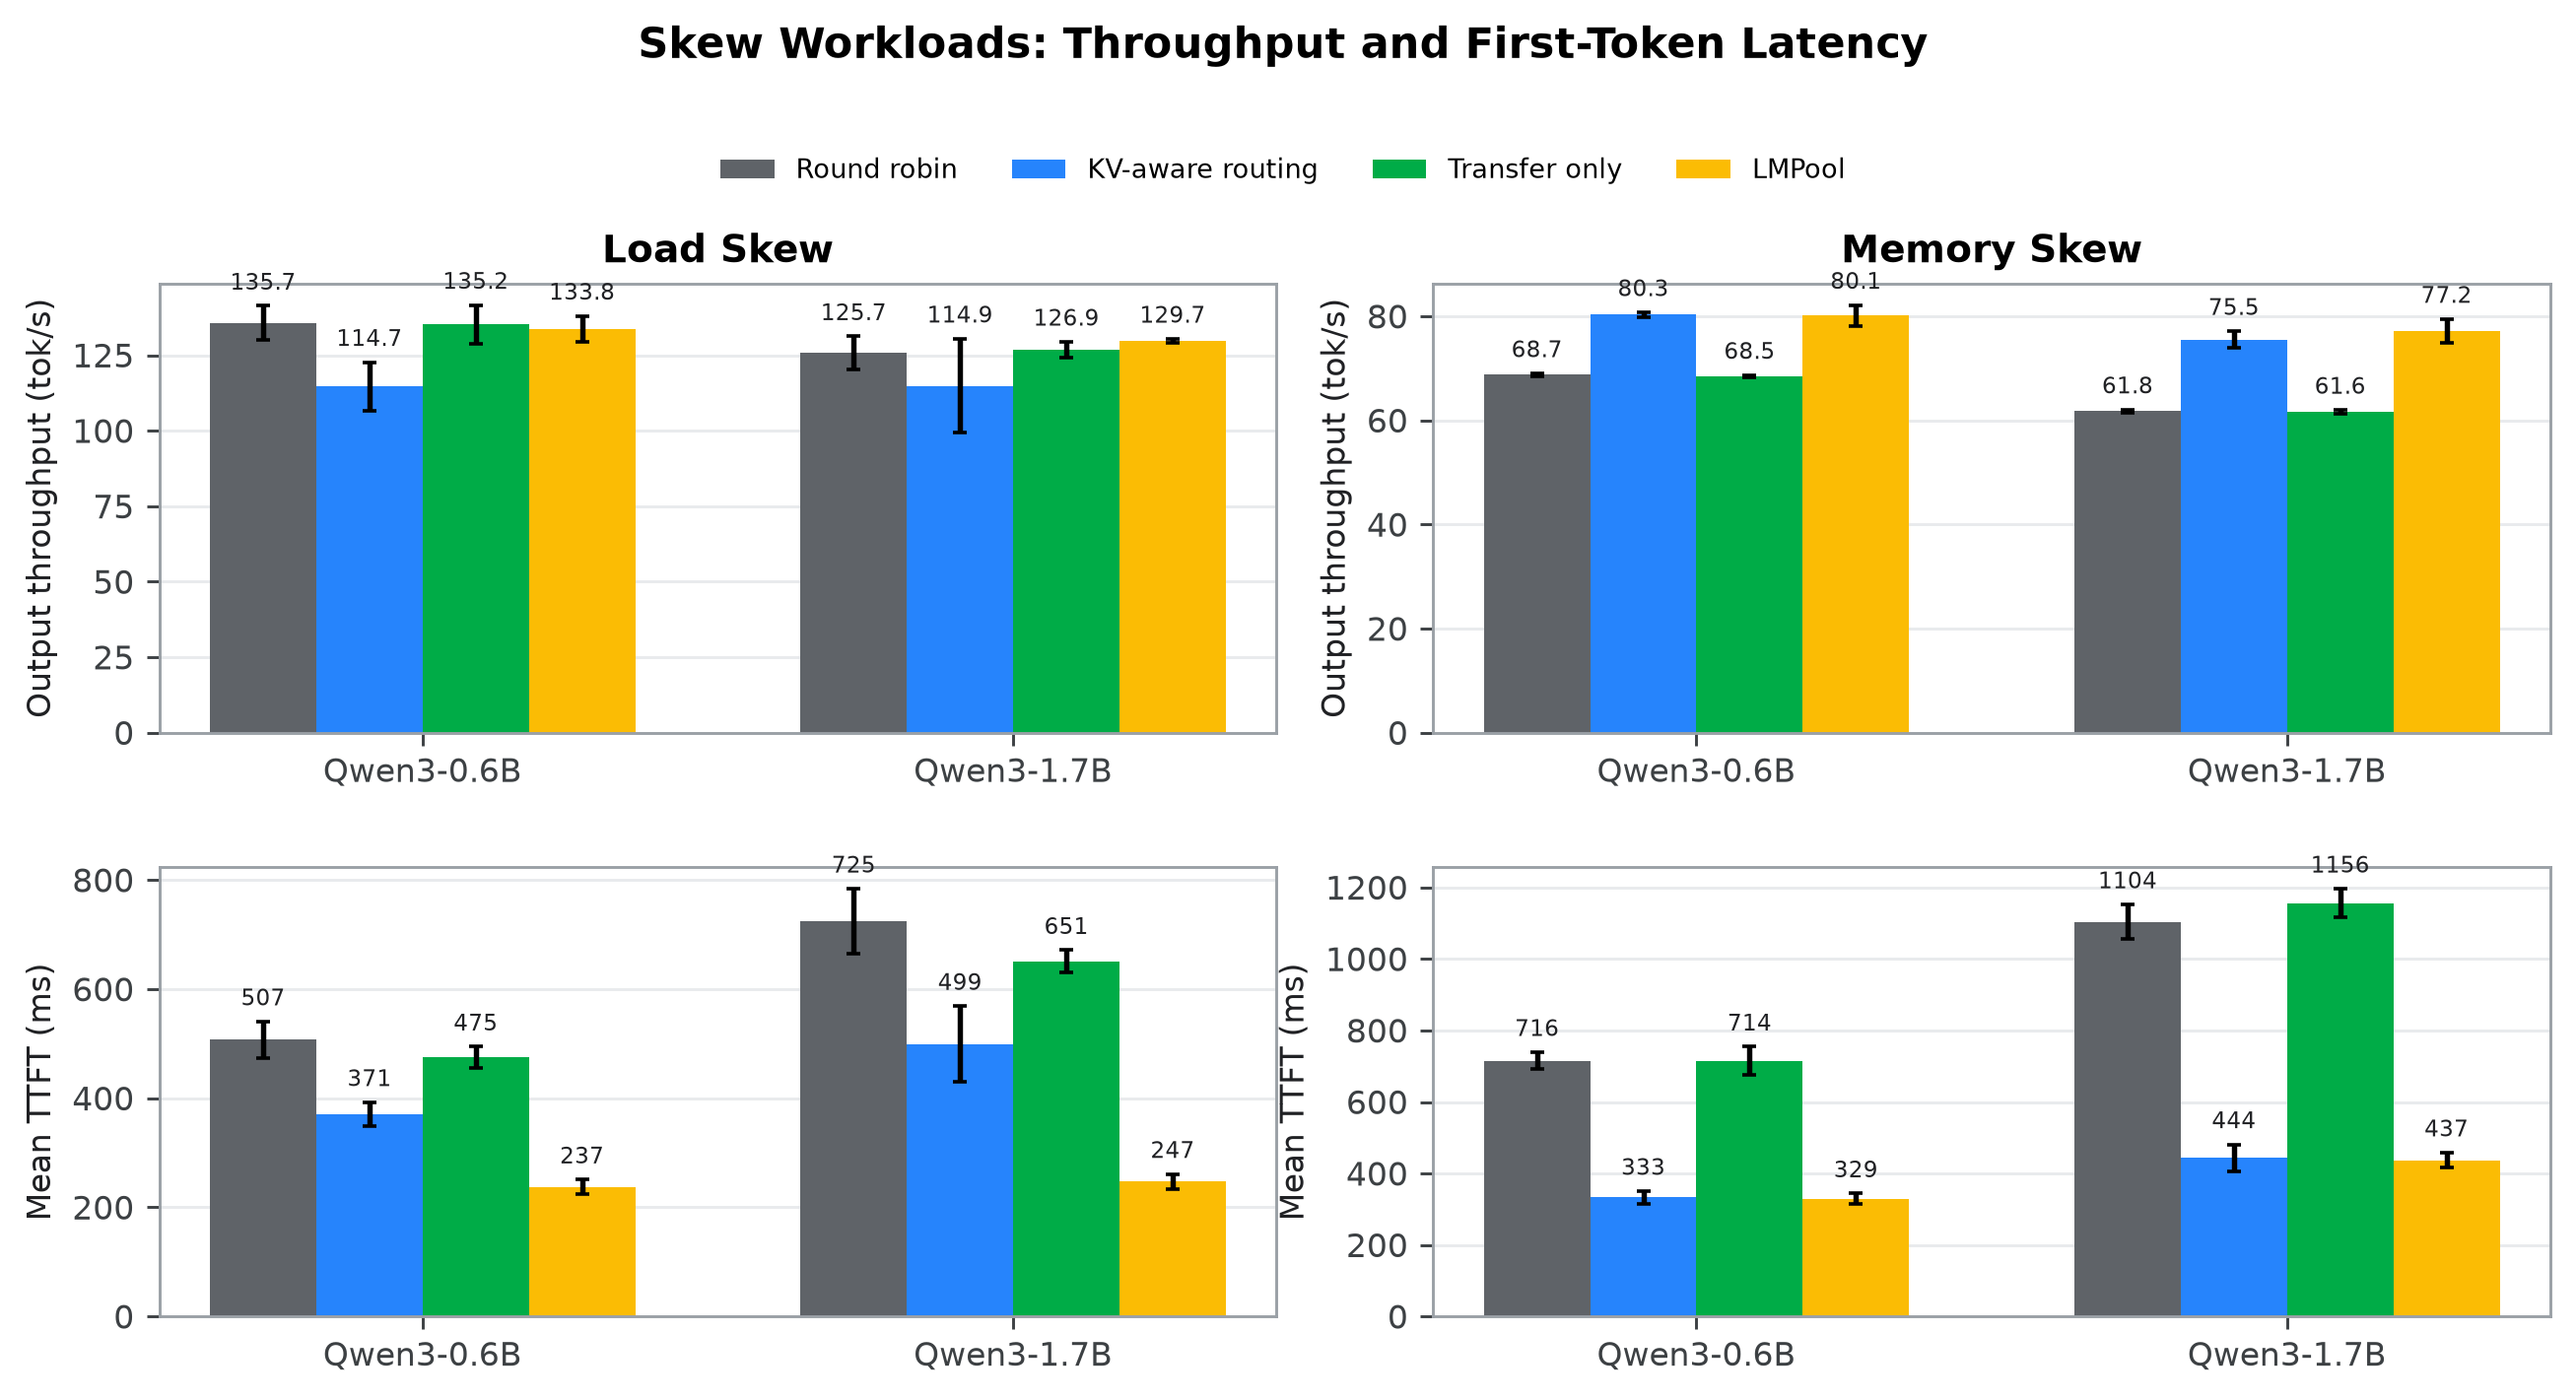
\includegraphics[width=\textwidth]{fig_suite_skew.png}
\caption{Load-skew 与 Memory-skew 工作负载上的 Throughput 和 Mean TTFT}\label{fig:suite-skew}\end{figure*}
\begin{figure*}[t]\centering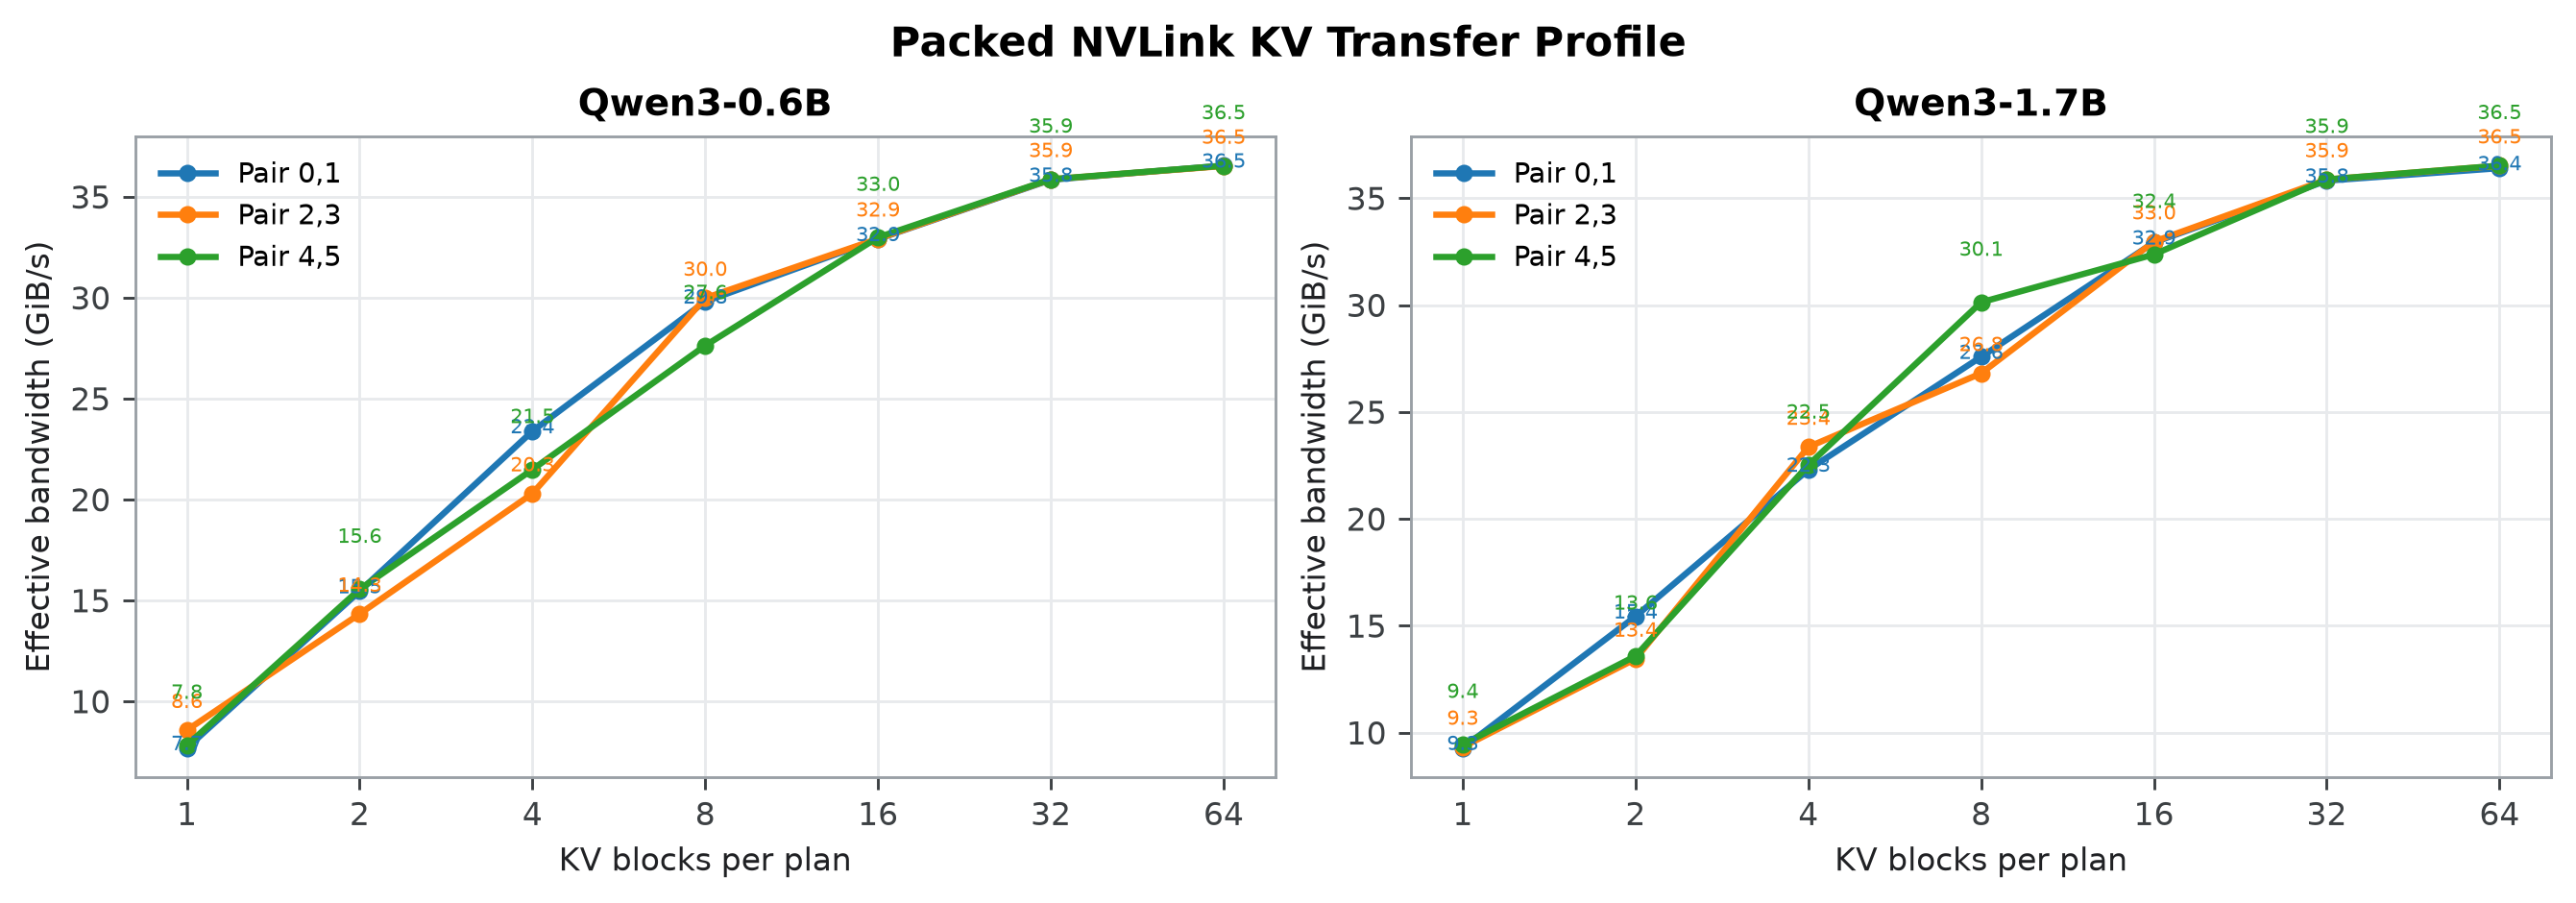
\includegraphics[width=0.92\textwidth]{fig_suite_transfer_profile.png}
\caption{跨 Direct GPU Pair 的打包 NVLink KV Transfer Profile}\label{fig:suite-transfer-profile}\end{figure*}

\subsection{Q1：Routing 改善长前缀服务}

\paragraph{Routing 收益随前缀长度增大。} 图~\ref{fig:suite-routing} 报告五次重复均值与 95\%
confidence interval。1x 时，routing 不改善 throughput：Qwen3-0.6B 从 164.7 变为 161.8~tok/s，
Qwen3-1.7B 从 148.9 变为 150.9~tok/s，TTFT 也不变或略高。匹配前缀太短，避免的 prefill 尚不足以
主导正常 scheduling variation。3x 与 5x 时，避免的 work 足以改变 service metric。5x 下，0.6B
throughput 从 43.63 提升到 48.77~tok/s，mean TTFT 从 536 降至 436~ms，mean E2E 从 2,743 降至
2,338~ms，P90 E2E 从 3,977 降至 3,140~ms，uncached prefill token 从 884,997 降至 354,821。
1.7B throughput 从 38.22 提升到 46.38~tok/s，mean TTFT 从 691 降至 517~ms，mean E2E 从 3,156
降至 2,479~ms，P90 E2E 从 4,903 降至 3,649~ms；对应 uncached prefill 降低 61.0\%。长前缀设置
下的改善超过报告的 run-to-run confidence interval。

\paragraph{Locality 被转换为节省的计算。} Routing sweep 中 request-level sharing bound 恒为 91.67\%，
但 token sharing 随共享前缀变长而增加。Router 不为 hit rate 添加独立奖励；更长的 contiguous match
降低 route cost 中的 missing-prefill term，因此同一 locality 直接减少 scheduled compute。5x 时效果
最强，两个模型同时改善 throughput 与所有报告 latency metric，而非只改善 cache-hit counter。

\subsection{Q2：批量 NVLink Transfer}

\paragraph{Data path 保持 KV 语义。} Microbenchmark 在两 rank 间 transfer 每个 layer 的 K/V tensor，
并逐 byte 验证 destination。它验证 packed tensor shape、byte count、dtype path 和 receive-side content，
说明 bandwidth measurement 对应 serving path 实际使用的 tensor，而非无关 communication primitive。
Microbenchmark 本身不证明端到端 serving benefit，因为它不包含 future reuse、queueing 或 model execution
interference。

\paragraph{大 plan 摊销固定 data-path cost。} 图~\ref{fig:suite-transfer-profile} 给出 serving path
使用的同一 packed tensor 的 effective bandwidth。Profile 覆盖三个 direct pair、两个模型和
1/2/4/8/16/32/64-block plan，逐 byte 验证 destination，并初始化 pair-specific P95 piecewise-linear
latency curve。64-block payload 约为 1.75~GiB，mean critical-path latency 约 48~ms；其 bandwidth 高于
small plan，是因为 gather、packing、communicator synchronization 与 scatter 被更多 K/V data 摊销，
不应将该曲线视为 raw-link measurement。Runtime plan 不限于采样 size，scheduler 按 payload 插值并以
已完成 operation 更新 pair-by-size residual。

\subsection{Q3：Background Copy 与 Placement Lease}

\paragraph{Load-skew trace 覆盖预期路径。} 请求共享率 98.44\% 的 load-skew trace 在三次 warm-up
后留下 target capacity。两个模型中，transfer-only 和完整 \sys{} 均完成三次 background placement，
copy 87 个 block；完整 \sys{} 随后通过 placement lease 路由 95 个请求，而 transfer-only 保持
round-robin admission。这表明 copied prefix 对后续 routing 可见，而非仅完成 data-path operation。

\paragraph{TTFT 改善，但 decode 可限制 E2E。} 对 0.6B，\sys{} 将 mean TTFT 从 round robin 的
507~ms 降至 237~ms，将 uncached prefill token 从 152,568 降至 41,208。相对 routing-only，TTFT
从 371 降至 237~ms，throughput 从 114.7 增至 133.8~tok/s，这与 lease routing 使用 copied replica、
而非让请求停在 original owner 的解释一致。但它仍略低于 round-robin throughput（133.8 对 135.7~tok/s），
且 mean E2E 更高（2,754 对 2,540~ms）。对 1.7B，\sys{} 将 throughput 从 125.7 增至 129.7~tok/s，
TTFT 从 725 降至 247~ms，P90 E2E 从 4,850 降至 4,071~ms；mean E2E 从 2,782 略增至 2,840~ms。
该 E2E trade-off 与 mean TPOT 增加一致：copied-prefix placement 降低 prefill delay，但当前 decode
scheduler 可能在 first token 后引入更多 contention。因此，load-skew 结果支持 background-copy
correctness 和显著 TTFT benefit，而非 universal mean-E2E claim。

\subsection{Q4：Capacity Offload 边界}

\paragraph{0.6B 验证 move-style release。} Memory skew 中，0.6B full-system 结果报告 35 个释放的
source block、两次 copy operation 和 true offload verification flag。Transfer-only 与 round robin
接近，throughput 为 68.47 对 68.75~tok/s，TTFT 为 714 对 716~ms，说明 movement 本身没有移除足够
work 以改善 service。Routing 是主要改善来源：它通过选择已有 local prefix chain，将 throughput 从
68.75 提升至 80.30~tok/s，TTFT 从 716 降至 333~ms；加入 move path 后为 80.11~tok/s 和 329~ms，
与 routing-only 在统计上接近。该实验验证安全的 capacity-release transaction，但未证明增量 throughput
收益。

\paragraph{1.7B 运行不构成 offload 结论。} 1.7B 结果记录了 moved block，但不满足完整 offload
verification predicate；其 full-system throughput/latency 与 routing-only 接近，confidence interval
重叠。因此，memory skew 被用于 implementation/safety result，而非证明 transfer-out 改善 serving
performance。Memory pressure 本身不能保证存在可复用、可执行且足够有价值的 transfer plan。

\section{讨论、局限与未来工作}

合成 phase structure 支持 causal attribution，但不能替代 production trace profiling。Background-placement
workload 使用 deterministic prompt identity 与 fixed replay order，而非已评估的 online forecast。未来
应 replay published 或 anonymized trace，并在选择 cache policy 前报告 prefix popularity、reuse distance、
prompt/decode distribution、session affinity transition、forecast accuracy 与 invalid-copy rate。

本研究仅使用一台 host、六张 consumer GPU 和两个小于 2B 参数且 KV geometry 相同的模型，未评估超过
六张 GPU 的 scale-out 或对 256-token KV block size 的 sensitivity。较小 block 可改变 fragmentation、
metadata cost、transfer-plan size 与 batching efficiency；较大模型改变 compute/transfer ratio，较大
NVLink fabric 改变 candidate selection。结果不应直接外推到 RDMA 或 PCIe-only cluster。

内部消融提供受控 mechanism comparison，但不比较完整 production serving stack。Kernel、scheduler、
prefix index 和 connector implementation 的差异使这些改善不能被解释为相对 vLLM、SGLang、Mooncake 或
LMCache 的 superiority。Versioned snapshot、transactional transfer、heartbeat 和 control-process restart
保持 metadata consistency 并支持 failure detection，但不实现 replicated consensus；launcher failure 会停止
service，worker failure 可能失去该 worker 上的 physical cache。

Model/pair-specific size curve 和 bucketed EWMA 捕获 payload scale 与 observed serving overhead。当前 runner
从 pair-specific P95 data-path profile 与 measured transaction residual 初始化 static estimate，只在出现
placement observation 前使用 zero-residual fallback。评估未报告 held-out prediction error，也未报告 safety
ratio/EWMA update sensitivity。Cost model 也不显式条件化 concurrent kernel、GPU clock rate 或 link contention；
compute state 的快速变化可能导致 estimate 不准确。

未来应在 public 或 anonymized multi-turn trace 上评估 online predictor，并报告 precision、recall、lead time
和 invalid-copy rate；应在相同 model、arrival process 与 KV budget 下比较至少一个 production serving engine，
并改变 model size、KV geometry、block size 与 GPU count。Transfer study 应报告 held-out prediction error，并
对 piecewise-linear profile、EWMA correction、safety ratio 与 no-gate policy 做 ablation。Production deployment
还需要 replicated control metadata 与 launcher failover，而非当前 single-control-process recovery model。

\section{相关工作}

\subsection{LLM Serving 与 Prefix Caching}

Orca 引入 transformer serving 的 iteration-level scheduling~\citep{ORCA}。vLLM 的 PagedAttention 将
KV allocation virtualize 为 block~\citep{vLLM}，SGLang 的 RadixAttention 为 structured program 组织
reusable prefix state~\citep{SGLang}。Sarathi-Serve 采用 chunked prefill 控制 prefill/decode interference
~\citep{SarathiServe}；DistServe 分离两个 phase，并在 TTFT/TPOT constraint 下优化 goodput~\citep{DistServe}。
这些系统建立 local execution/scheduling 的背景。\sys{} 则研究 data-parallel replica 间的 admission-time
placement，它们可通过 direct NVLink copy KV block。

\subsection{Distributed 与 Tiered KV Cache}

Mooncake 提出 KV-cache-centric disaggregated architecture，以 distributed storage capacity 换取更少的
prefill computation~\citep{Mooncake}。vLLM 与 Mooncake Store 的较新集成通过 GPUDirect RDMA 和 distributed
DRAM/SSD service 在 instance 间 pool KV state。其 agentic trace 官方评估在 12 张 GB200 上报告 3.8$\times$
更高 throughput、46$\times$ 更低 P50 TTFT 和 8.6$\times$ 更低 E2E latency；synthetic scale-out 在 60 GPU
上保持超过 95\% cache hit rate~\citep{MooncakeStore}。该集成可在 scheduling 时查询 block hash，但作者将完整
cache-aware routing 与 multi-node NVLink support 列为 future work。PegaFlow 则把 cache ownership 放在 long-lived
Rust service，结合 pinned host DRAM、one-sided RDMA read 和 local SSD；vLLM/Novita 报告在八个 Qwen3-8B
instance 共享一个 fixed host-cache budget 时 throughput 提升 56\%，deduplicated TP8 MLA KV 时提升 72\%，
8-NIC RDMA cluster 中至少 1~GiB object 的平均 read bandwidth 为 194~GB/s~\citep{PegaFlow}。

MemServe 提供 elastic memory pool 和 global prompt-tree scheduler 用于 disaggregated serving~\citep{MemServe}；
CachedAttention 在 hierarchy 中保存 multi-turn KV state，并与 compute overlap load/save~\citep{CachedAttention}；
CacheGen 压缩 KV state 以在受限 link 上加速 context loading~\citep{CacheGen}；LMCache 提供跨 engine 与
storage/communication backend 的 reusable cache layer~\citep{LMCache}。这些系统强调 capacity、persistence 或
cross-node visibility。\sys{} 关注更窄的 scale-up setting：由 direct NVLink 连接的 data-parallel replica 上
物理局部的 HBM cache。

\subsection{Migration 与 Multi-GPU Memory Balance}

Aqua 在 bursty memory pressure 下利用由 NVLink/NVSwitch 连接 GPU 的 spare memory，对 inference state 做
page，以支持 preemptive、time-sliced serving。在八张 H100 上，Aqua 报告最高 20$\times$ 的 responsiveness
提升和单个 long prompt 最高 4$\times$ throughput 提升~\citep{Aqua}。Aqua 因而为 active inference state
提供 fluidity，但不按 content-addressed prefix ownership 路由请求。Llumnix 通过迁移 request 支持 dynamic
rescheduling 与 defragmentation~\citep{Llumnix}；MELL 联合考虑 multi-GPU KV load 与 request migration cost
~\citep{MELL}。这些研究表明 state movement 是有成本的 scheduling operation，而非总是有利的 fallback。
\sys{} 的区别在于使用 content-addressed prefix chain、copy-based replication 与 placement lease，使 source
与 destination 都可服务未来请求。

表~\ref{tab:related-principles} 区分常被统称为 ``distributed KV cache'' 的三类关切。Locality-aware
placement 将请求分配到已有相关 prefix 的 GPU；fluidity-aware placement 在当前位置不再匹配需求时移动 state；
coupled admission 在 routing/transfer 间选择前比较 recomputation、queueing、capacity 与 measured transfer cost。
表中 ``Partial'' 表示 metadata lookup，但没有公开的 policy 联合考虑 locality、load、routing 与 transfer
admission。比较并不表示 \sys{} 替代 durable 或 cross-node cache system，而是说明在所列系统中，\sys{}
将三种 decision 集成在 serving scheduler 内。

\begin{table}[!htbp]\centering\scriptsize
\caption{按 Locality-Aware Placement、Fluidity Mechanism、Durable Capacity 和 Coupled Admission 的 KV-Cache 系统比较}
\label{tab:related-principles}\setlength{\tabcolsep}{1.5pt}
\begin{tabularx}{\linewidth}{@{}L{0.10\linewidth}Y Y Y L{0.10\linewidth}Y@{}}\toprule
系统 & 主要范围 & Locality-aware request placement & Fluidity mechanism/path & Durable/multi-tier pool & Coupled route--transfer admission\\\midrule
Mooncake Store~\citep{MooncakeStore} & Cluster-wide agentic prefix reuse & Partial：hash lookup 辅助 scheduling，完整 cache-aware routing 仍是 future work & GPU HBM 与 distributed cache worker 间异步 GPUDirect RDMA & 是：DRAM/SSD & 无公开模型比较 recomputation 与 transfer cost\\
PegaFlow~\citep{PegaFlow} & External、process-independent KV lifetime/sharing & 否：vLLM 保留 request scheduling，global index 定位 remote hit & Local CUDA IPC、cross-node one-sided RDMA；cold block 使用 SSD & 是：pinned DRAM、remote DRAM、SSD & 否；TinyLFU 管理 cache admission，不在 routing/transfer 间选择\\
Aqua~\citep{Aqua} & GPU-memory burst 下 responsive preemption & 无 content-addressed prefix routing & 经 NVLink/NVSwitch 将 inference state page 到 spare GPU HBM & 否：volatile GPU HBM & 基于 memory pressure，而非 expected future prefix reuse\\
\sys{} & Data-parallel GPU replica 间的 KV locality/fluidity & 是：最长 contiguous prefix 与 load/effective capacity 联合评分 & 在 configured NVLink pair 的 peer HBM 间 copy/move & 否：volatile GPU HBM & 是：先 route，再基于 measured cost 与 expected reuse 准入 transfer\\\bottomrule
\end{tabularx}\end{table}

\section{结论}

\sys{} 通过 global routing 协调物理局部 KV cache 以获得 cache locality，并仅在 expected benefit 覆盖 cost 时
使用 pair-local NVLink transfer 获得 cache fluidity。实现将 authoritative control process 与 per-GPU data
process 分离，并在 configured direct pair 上结合 versioned metadata 与 transactional block movement。实验
在两个模型的长共享前缀下显示稳定 routing gain，验证 load skew 中的 background copy/lease routing 及 0.6B
memory skew 中的 source-block release，并给出当前边界：completed movement 本身不保证更低 E2E latency 或更高
throughput。

\section*{致谢}
感谢 Yijun Sun、Kai Chen 教授的项目指导，以及 Mini-vLLM 作者提供基础推理引擎。

\bibliographystyle{unsrtnat}
\bibliography{references}

\ifXeTeX\else\end{CJK*}\fi
\end{document}
